\documentclass{beamer}
%\documentclass[handout]{beamer}
%\usepackage{pgfpages}
%\pgfpagesuselayout{2 on 1}[a4paper,border shrink=5mm]

\usepackage{verbatim}
\usepackage{amssymb}
\usepackage{amsmath}

\mode<presentation>
{
  \usetheme{Singapore}  %Warsaw}  %CambridgeUS}
  
  \setbeamercovered{transparent}
  }


\usepackage[english]{babel}
\usepackage[latin1]{inputenc}
\usepackage{times}
\usepackage[T1]{fontenc}
\newcommand{\bs}{\boldsymbol}
\newcommand{\mb}{\mathbf}
\newcommand{\x}{\mathbf{x}}
\newcommand{\X}{\mathbf{X}}
\newcommand{\y}{\mathbf{y}}
\newcommand{\Y}{\mathbf{Y}}

\title[Descriptive Statistics/Questions with Linear Regression] {Descriptive Statistics/Questions with Linear Regression}

%\subtitle
%{Descriptive Questions} 

%\author[Adam Glynn]{Adam Glynn}
%\institute[Harvard University]{Harvard University} 

\date{August 31 and September 5 2017}

\subject{Talks}

\AtBeginSection[]
{
  \begin{frame}<beamer>
    \frametitle{Outline}
    \tableofcontents[currentsection,currentsubsection]
  \end{frame}
}


\AtBeginSubsection[]
{
  \begin{frame}<beamer>
    \frametitle{Outline}
    \tableofcontents[currentsection,currentsubsection]
  \end{frame}
}

\begin{document}

\begin{frame}
  \titlepage
\end{frame}




\begin{frame}
  \frametitle{Outline}
  \tableofcontents
 
\end{frame}

%%%%%%%%%%%%%%%%%%%%


\frame{
\frametitle{Plan for Today and Tuesday}

\begin{itemize}
\item Descriptive Inference is about using samples to answer questions about populations. \pause
\item There are many possible questions we might have about populations.  \pause
\item To simplify the discussion, we will start by analyzing the case where we observe the entire population (i.e., a census) and no sampling is necessary.  \pause
\item This is sometimes known as descriptive statistics, although this term is often used with reference to a sample.
\end{itemize}

}


\section{Describing Univariate and Multivariate Populations}

\frame{
\frametitle{Description}

\begin{itemize}
\item Two weeks ago we considered a population with a single variable that took only one of two values (0 or 1).  \pause
\item This week we consider some variables that take many values. \pause
\item This week we consider some populations that have more than one variable.
\end{itemize}

}


\frame{
\frametitle{Example: Epstein and Mershon SCOTUS data}

\begin{itemize}
\item Data on 27 justices from the Warren, Burger, and Rehnquist courts (can be interpreted as a census)  \pause
\item Percentage of votes in liberal direction for each justice in a number of issue areas  \pause
\item Segal-Cover scores for each justice  \pause
\item Party of appointing president
\end{itemize}

}

\frame{
\frametitle{Describing Univariate Data}

\begin{figure}[ht] \centering
        \scalebox{.4}{
\includegraphics{CLhist.pdf}}
\end{figure}


}

\frame{
\frametitle{Describing Bivariate Data}

\begin{figure}[ht] \centering
        \scalebox{.4}{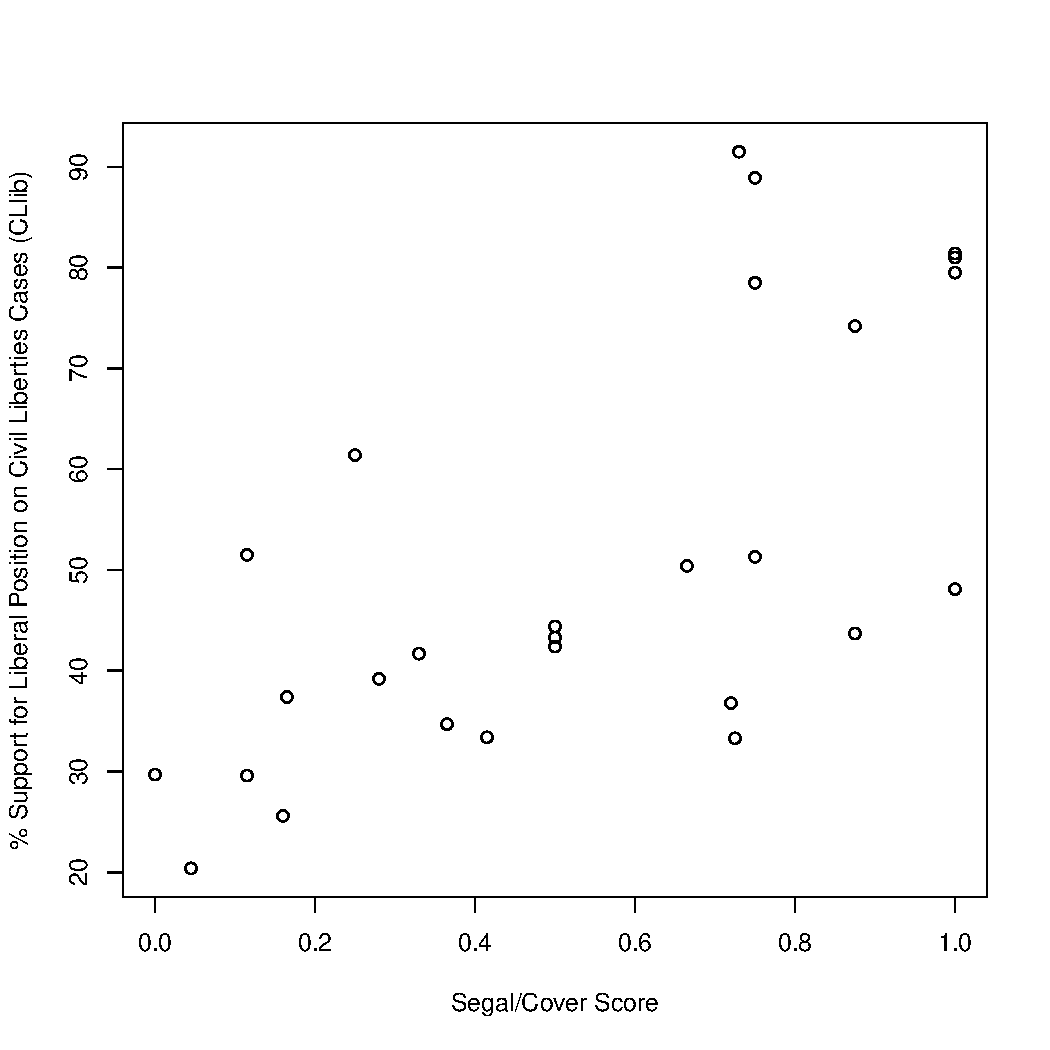
\includegraphics{scat2d.pdf}}
\end{figure}


}


\frame{
\frametitle{Describing Bivariate Data}

\begin{figure}[ht] \centering
        \scalebox{.4}{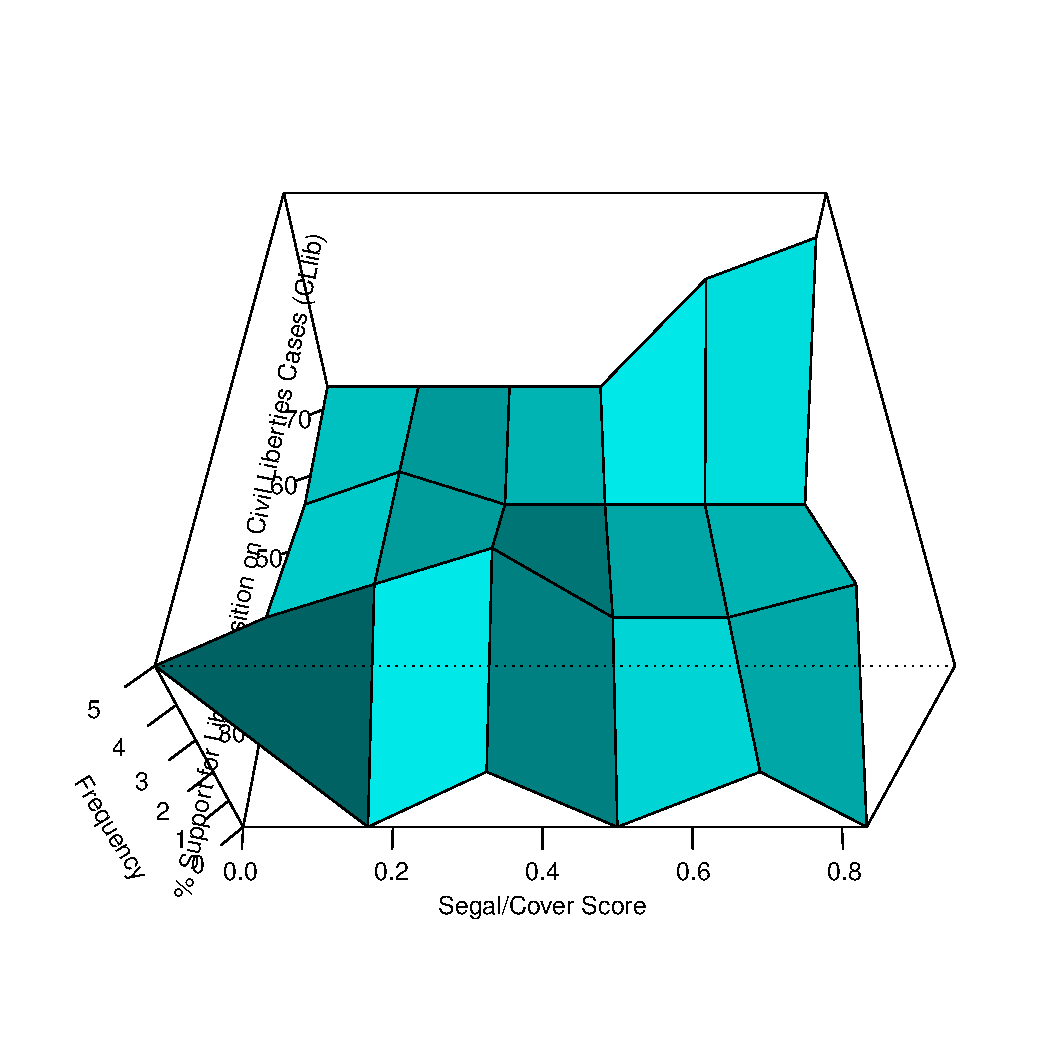
\includegraphics{hist2d.pdf}}
\end{figure}


}


\frame{
\frametitle{Describing Trivariate Data}

\begin{figure}[ht] \centering
        \scalebox{.4}{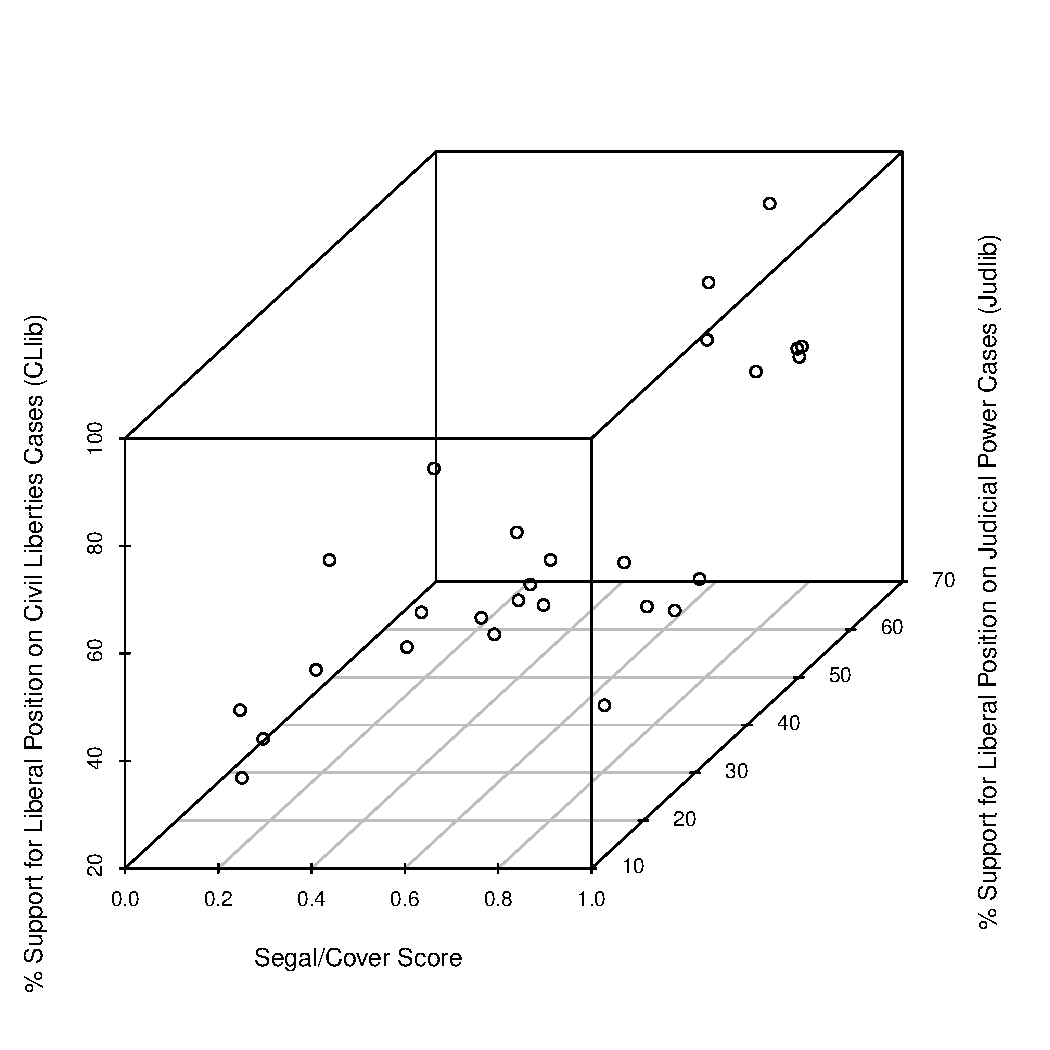
\includegraphics{scat3d.pdf}}
\end{figure}

}



\frame{
\frametitle{Summarization}

\begin{itemize}
\item Even for univariate data, we may want to focus on one or two characteristics of the population instead of describing it in its entirety. \pause
\item We typically focus on measures of center and spread.\pause
\item We will discuss the rational for this over the coming weeks.
\end{itemize}
}


\frame{
\frametitle{Univariate Activity}

\begin{figure}[ht] \centering
        \scalebox{.4}{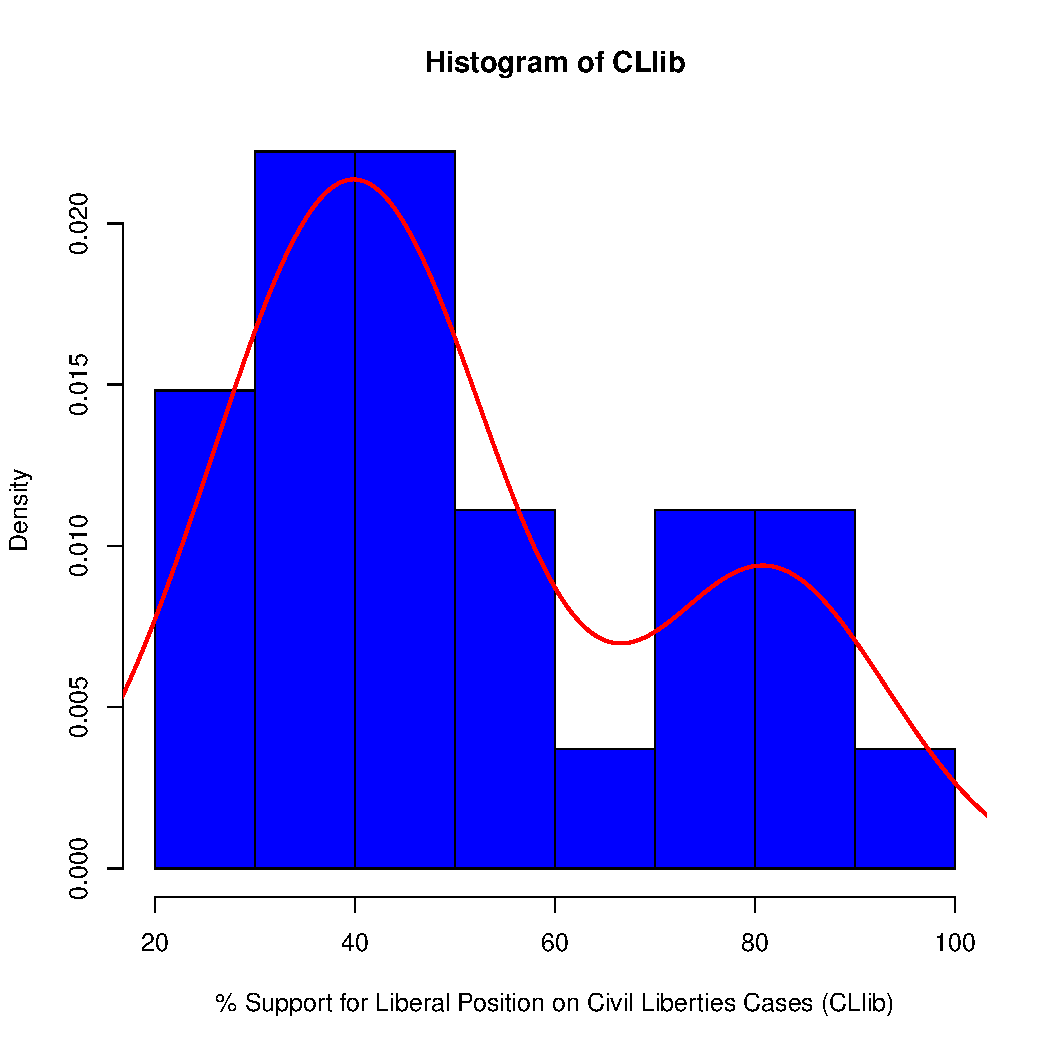
\includegraphics{CLhistAct.pdf}}
\end{figure}

}

\frame{
\frametitle{Univariate Activity Solution}

\begin{figure}[ht] \centering
        \scalebox{.4}{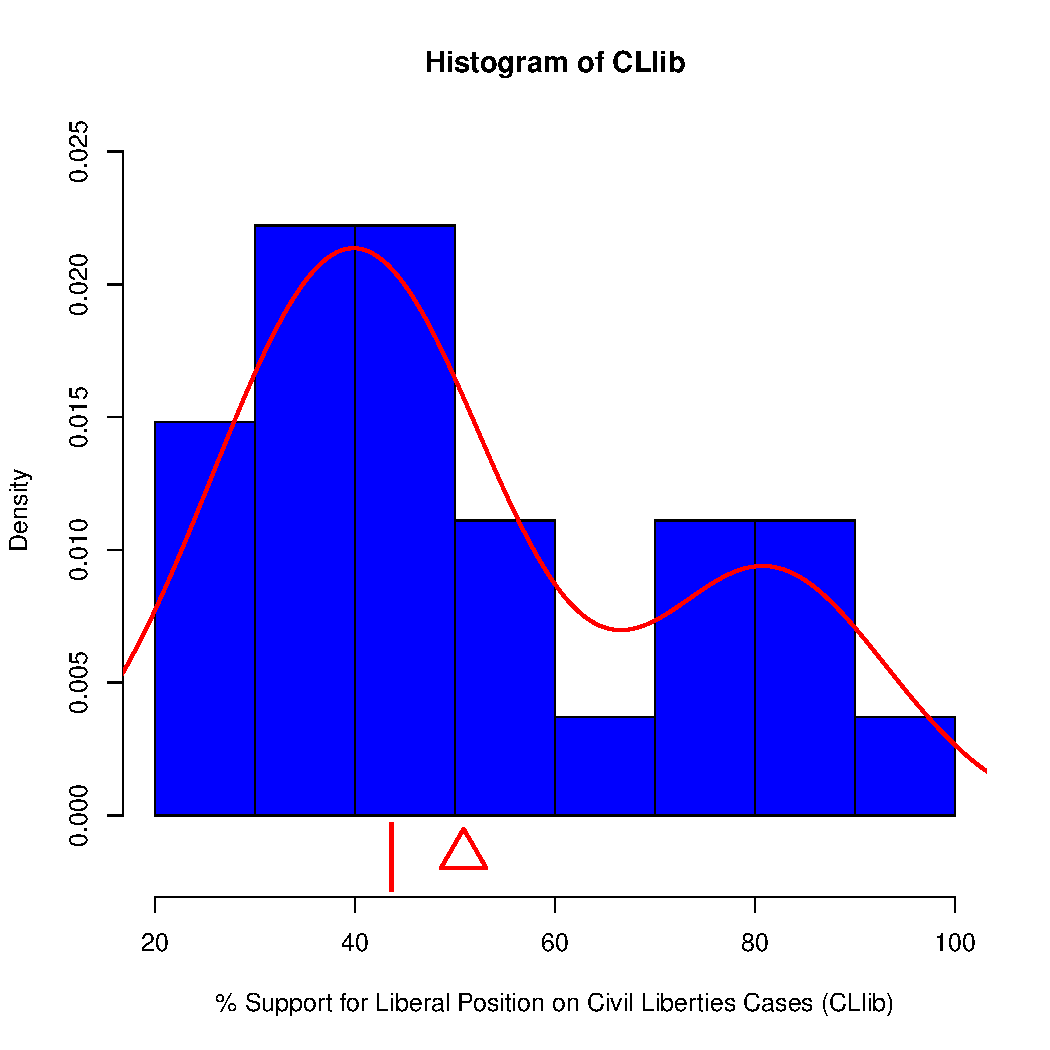
\includegraphics{CLhistActSol.pdf}}
\end{figure}

}


\frame{
\frametitle{Why Do We Focus on Means?}


\begin{itemize}
\item Population means ($\bar{y} = \frac{1}{N}\sum_{i=1}^N  y_i$) often provide a ``good'' summary of the center of the data (and it is relatively easy to tell when they provide bad summaries).  \pause
\item The accuracy of means is relatively easy to describe.  \pause
\item Randomized experiments only identify average causal effects (as do regression and matching when the appropriate assumptions hold).
\end{itemize}

}


\frame{
\frametitle{The Mean as a Least Squares Summary}

Suppose we want to pick a single number ($m$) for the middle of the data that summarizes all the values for $y$, by minimizing the sum of squared residuals (i.e., least squares).
$$
SSR(\tilde{m}) = \sum_{i=1}^N (y_i - \tilde{m})^2.
$$
\pause

One way to calculate the least squares estimator
\begin{enumerate}
  \item Calculate the derivative of $SSR$ with respect to $\tilde{m}$
  \item Set the derivative equal to 0
  \item Solve for $m$
\end{enumerate}

}

\frame{
\frametitle{The Objective Function for SSR CLlib}
\begin{figure}[ht] \centering
        \scalebox{.4}{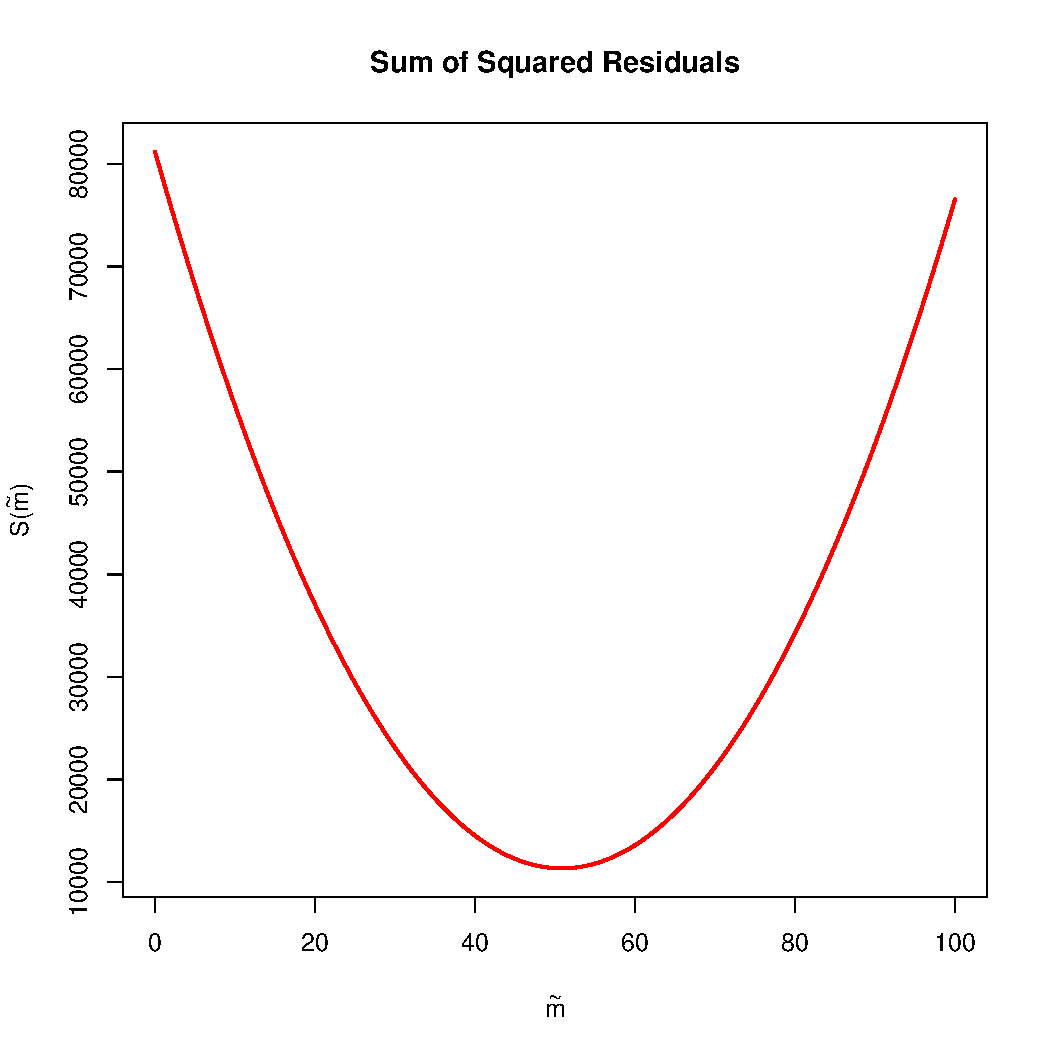
\includegraphics{objectiveFunction1.pdf}}
\end{figure}

}

\frame{

\begin{enumerate}
\item \begin{align*}
SSR(\tilde{m}) 
  &= \sum_{i=1}^N (y_i -
  \tilde{m})^2\\
  &= \sum_{i=1}^N (y_i^2 - 2 y_i \tilde{m} + \tilde{m}^2)
\end{align*} 
 $$
\frac{\partial SSR(\tilde{m})}{\partial
  \tilde{m}} = \sum_{i=1}^N (-2 y_i + 2 \tilde{m})
$$
\end{enumerate}


\vspace{3cm}
}

\frame{
\frametitle{The Slope of the Tangent Line for SSR CLlib}
\begin{figure}[ht] \centering
        \scalebox{.4}{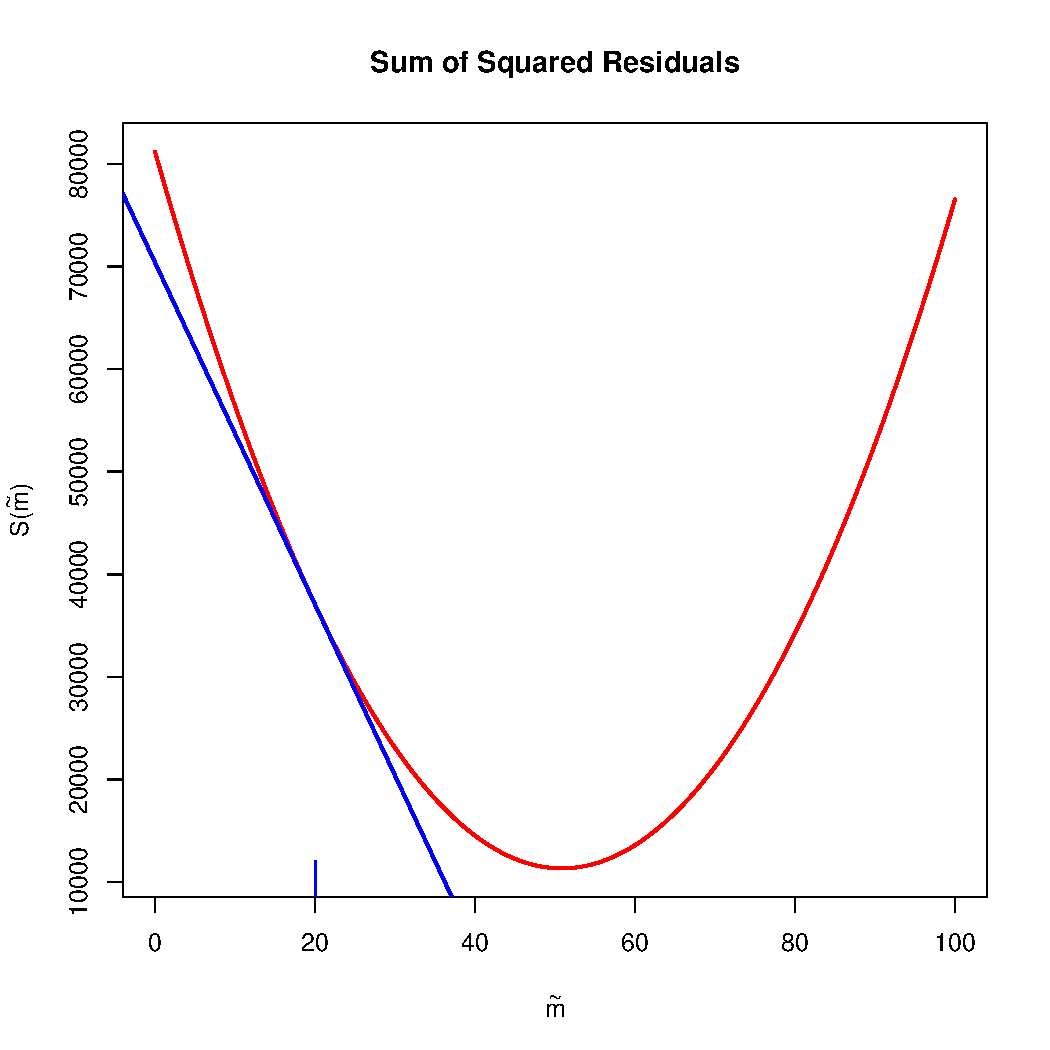
\includegraphics{objectiveFunction2.pdf}}
\end{figure}

}

\frame{
\frametitle{The Slope of the Tangent Line for SSR CLlib}
\begin{figure}[ht] \centering
        \scalebox{.4}{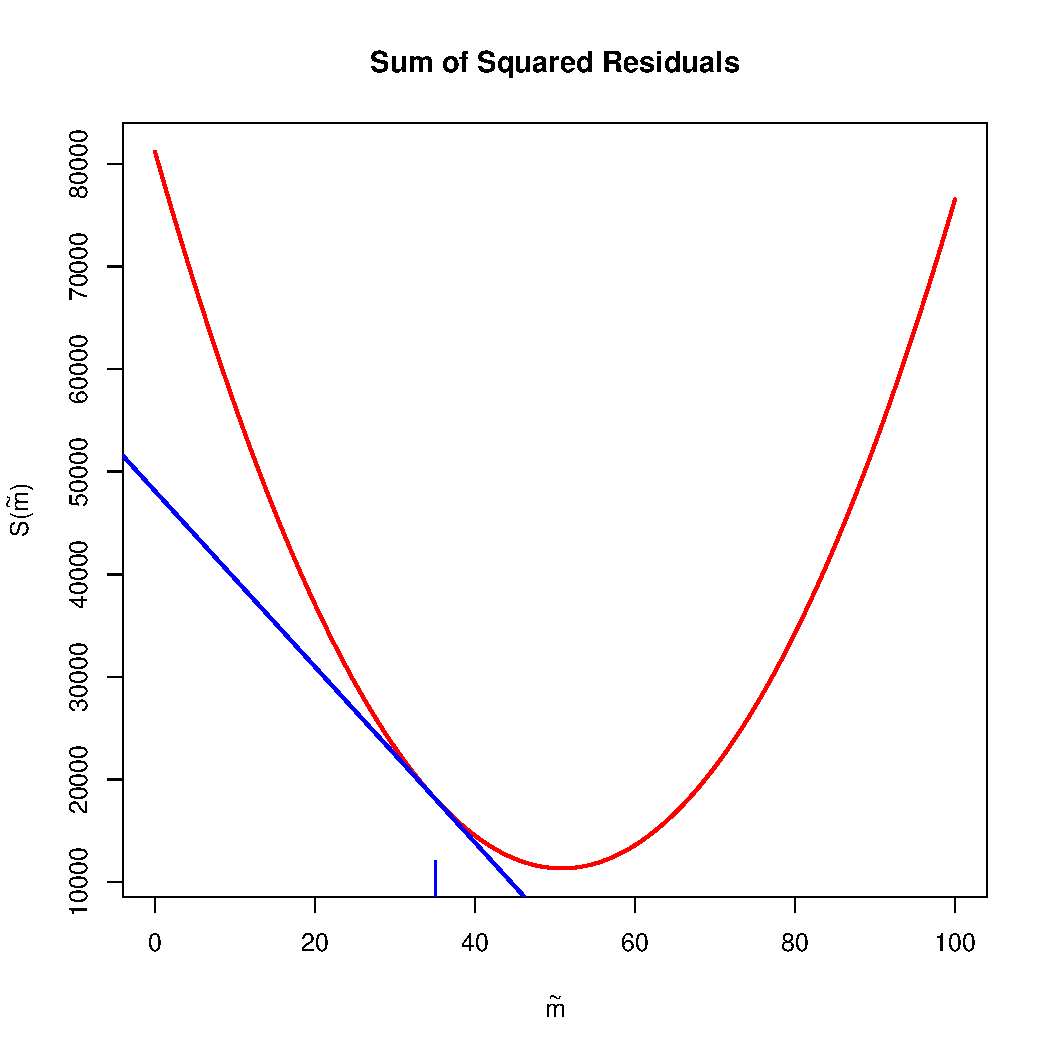
\includegraphics{objectiveFunction3.pdf}}
\end{figure}

}

\frame{
\frametitle{The Slope of the Tangent Line for SSR CLlib}
\begin{figure}[ht] \centering
        \scalebox{.4}{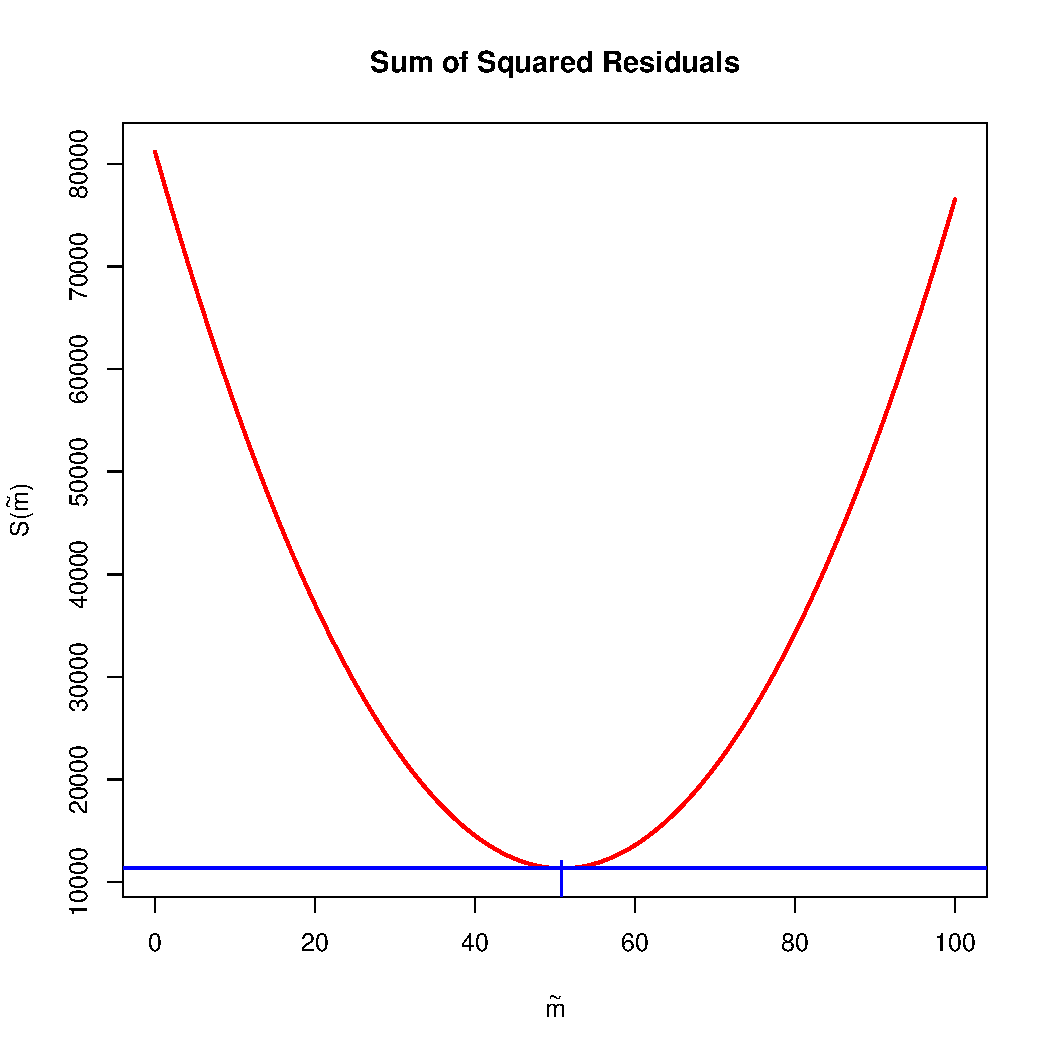
\includegraphics{objectiveFunction4.pdf}}
\end{figure}

}


\frame{

\begin{enumerate}
\item \begin{align*}
SSR(\tilde{m}) 
  &= \sum_{i=1}^N (y_i -
  \tilde{m})^2\\
  &= \sum_{i=1}^N (y_i^2 - 2 y_i \tilde{m} + \tilde{m}^2)
\end{align*} 
 $$
\frac{\partial S(m)}{\partial
  \tilde{m}} = \sum_{i=1}^N (-2 y_i + 2\tilde{m})
$$

\item $$
0 = \sum_{i=1}^N (-2 y_i + 2 m)
$$
\item $$
m = \frac{1}{N}\sum_{i=1}^N  y_i 
$$
\end{enumerate}
\vspace{.4cm}
Therefore, the population mean is a least squares summary.

}

\frame{
\frametitle{Variance and Standard Deviation}

\begin{itemize}
\item Mean is the least squares predictor in terms of SSR.
\item How small is ``least'' (i.e., how much spread around the mean)?
\item Variance and Standard Deviation are useful transformations of SSR for the mean.
\end{itemize} \pause

Population Variance
\begin{align*}
S^2 &= \frac{\sum_{i=1}^N (y_i-\bar{y})^2}{N-1} \\ 
&=  \frac{SSR}{N-1}
\end{align*} \pause

Population Standard Deviation
\begin{align*}
S &= \sqrt{S^2}
\end{align*}

}

\frame{
\frametitle{Mean and Standard Deviation}

\begin{figure}[ht] \centering
        \scalebox{.4}{
\includegraphics{CLhistMSD.pdf}}
\end{figure}


}


\section{Description with Linear Regression}


\frame{
\frametitle{Conditional Means}

\begin{itemize}
\item In this class, we focus on a single ``outcome'' variable. 
\item All additional variables adjust how we consider the outcome, often by conditioning.
\item Typically, we consider the mean of $y$ conditional on values of other variables.
\end{itemize}

}

\frame{
\frametitle{Mean CLlib Conditional on Party}

\begin{figure}[ht] \centering
        \scalebox{.4}{\includegraphics{partyMean.pdf}}
\end{figure}


}

\frame{
\frametitle{Linear Conditional Mean Function (LCMF)}

\begin{figure}[ht] \centering
        \scalebox{.4}{
\includegraphics{lmBin.pdf}}
\end{figure}


}

\frame{
\frametitle{What about a continuous explanatory variable?}

\begin{center}
\includegraphics<1>[width=7.25cm]{justicePlot1.pdf}
\includegraphics<2>[width=7.25cm]{justicePlot2.pdf}
%\includegraphics<3>[width=7.25cm]{justicePlot1.pdf}
%\includegraphics<4>[width=7.25cm]{justicePlot3.pdf}
\includegraphics<3>[width=7.25cm]{justicePlot4.pdf}
\end{center}


}




\frame{
\frametitle{Fitted Values and Residuals}

\begin{itemize}
\item Fitted Values from LCMF: $\alert{\hat{y}_i} = B_0 + B_1 x_i$ for $i=1,...,N$ 
\item Residuals from Fitted Values:  $\textcolor{green}{e_i} = y_i - \hat{y}_i$ for $i=1,...,N$
\end{itemize}

\vspace{-.3cm}

\begin{center}
\includegraphics<1>[width=7cm]{fitted.pdf}
\includegraphics<2>[width=7cm]{fitted2.pdf}
\includegraphics<3>[width=7cm]{residuals.pdf}
\end{center}
}

\frame{
\frametitle{Minimizing the Residuals}

%Intuitively, we want to "minimize" the residuals. However, any line through the point of averages

\begin{itemize}
\item Let $\tilde{B}_0$ and $\tilde{B}_1$ be possible values for $B_0$ and $B_1$ respectively,
    \item \emph{Least Squares (LS) regression}: 
    $$
    (B_0, B_1) =   
     \underset{\tilde{B}_0, \tilde{B}_1}{\textrm{argmin}}
    \sum_{i=1}^N (y_i - \tilde{B}_0 - x_i \tilde{B}_1)^2
    $$ 
\end{itemize}

}

\frame{
\frametitle{Simple Regression Activity}

\begin{center}
\includegraphics<1>[width=7.25cm]{simRegAct.pdf}
\includegraphics<2>[width=7.25cm]{simRegActSol.pdf}

\end{center}

}

\frame{
\frametitle{Choosing Slope and Intercept to Minimize SSR}

\begin{figure}[ht] \centering
        \scalebox{.45}{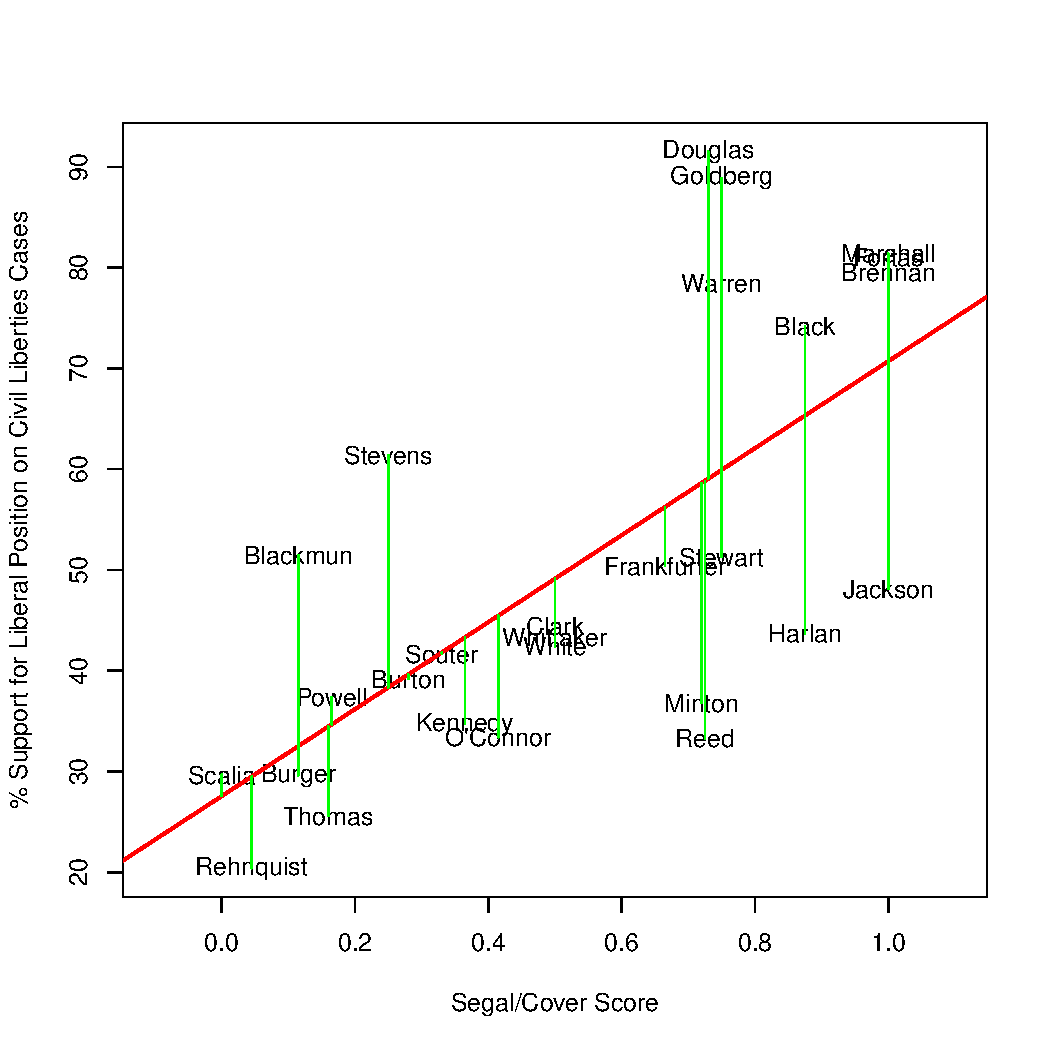
\includegraphics{residuals.pdf}}
\end{figure}

}


\frame{
\frametitle{Deriving the Linear Least Squares Estimator}

Let $\tilde{B}_0$ and $\tilde{B}_1$ be possible values for $B_0$ and $B_1$ respectively, and 
$$
S(\tilde{B}_0, \tilde{B}_1) = \sum_{i=1}^N (y_i -
\tilde{B}_0 - x_i \tilde{B}_1)^2.
$$


\begin{enumerate}
  \item  Take partial derivatives of $S$ with respect to
    $\tilde{B}_0$ and $\tilde{B}_1$. 
  \item Set each of the partial derivatives to 0
  \item Substitute $B_0$ and $B_1$ for
    $\tilde{B}_0$ and $\tilde{B}_1$ and solve for
    $B_0$ and $B_1$
\end{enumerate}

}


%\frame{
%\frametitle{The Objective Function for OLS}
%\begin{figure}[ht] \centering
%        \scalebox{.4}{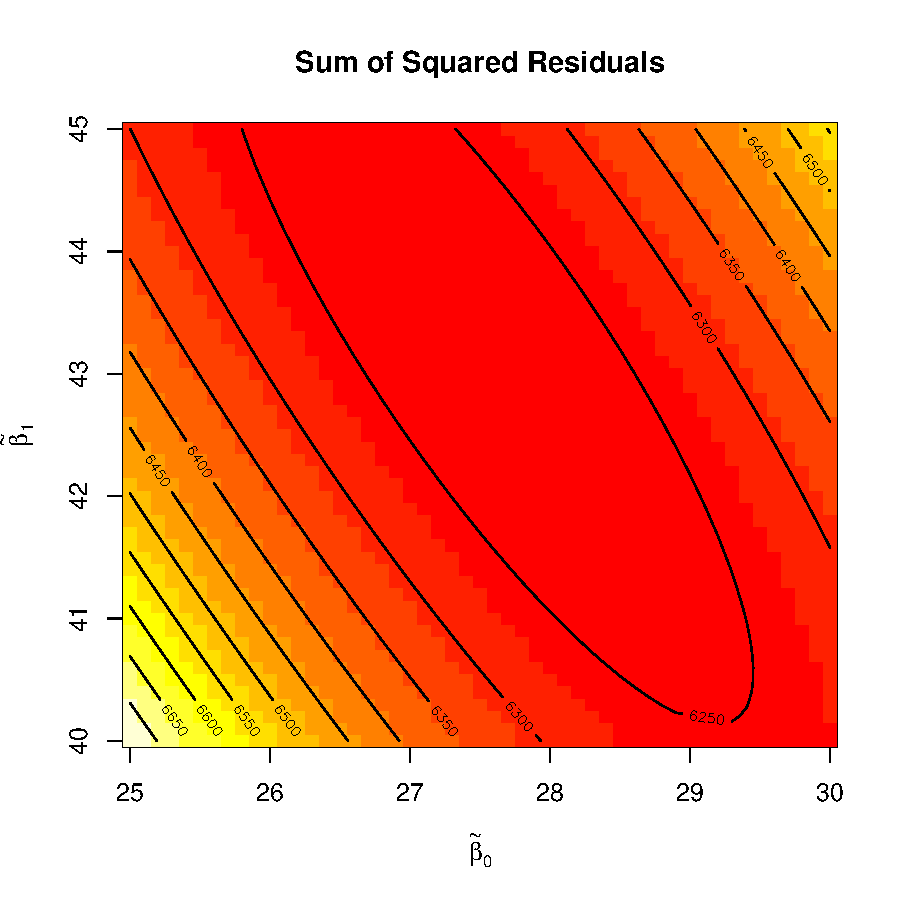
\includegraphics{OLSobjectiveFunction1.pdf}}
%\end{figure}
%
%}
%
%\frame{
%\frametitle{The Objective Function for OLS}
%\begin{figure}[ht] \centering
%        \scalebox{.4}{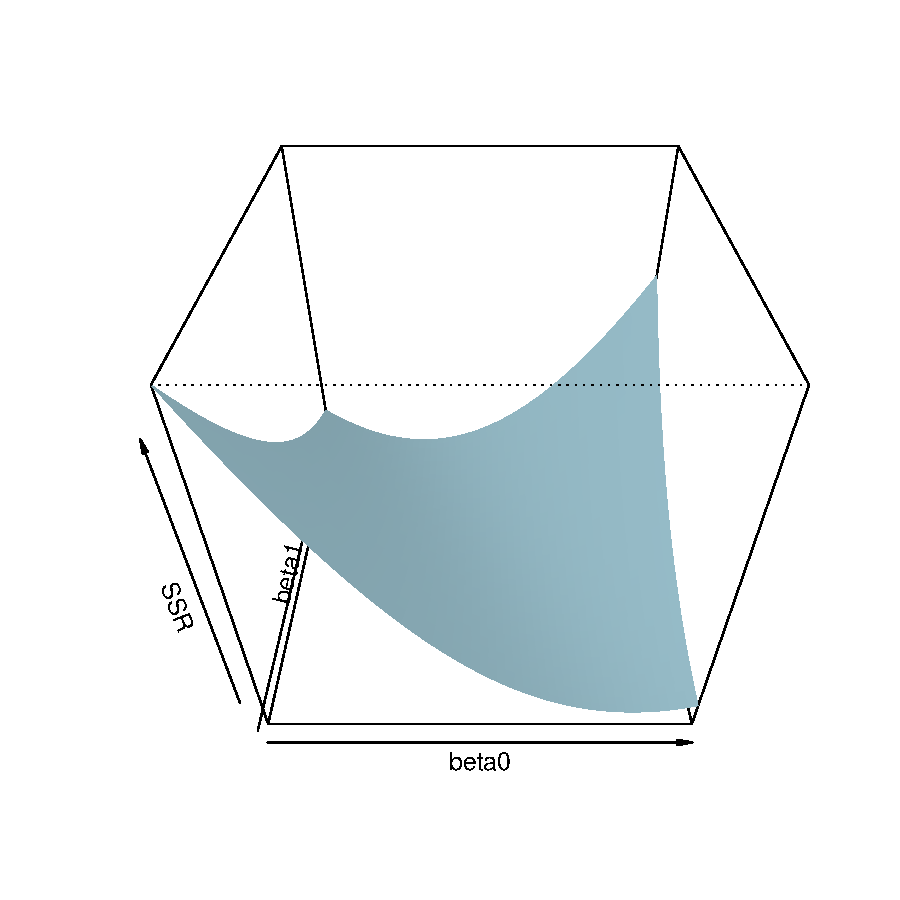
\includegraphics{OLSobjectiveFunction2.pdf}}
%\end{figure}
%
%}


%\frame{

%\begin{align*}
%S(\tilde{\beta}_0, \tilde{\beta}_1) 
%  &= \sum_{i=1}^n (y_i -
%  \tilde{\beta}_0 - x_i \tilde{\beta}_1)^2\\
%  &= \sum_{i=1}^n (y_i^2 - 2 y_i \tilde{\beta}_0 - 2 y_i
%  \tilde{\beta}_1 x_i + \tilde{\beta}_0^2 + 2 \tilde{\beta}_0
%  \tilde{\beta}_1 x_i + \tilde{\beta}_1^2 x_i^2)
%\end{align*} 

%

%$$
%\frac{\partial S(\tilde{\beta}_0, \tilde{\beta}_1)}{\partial
%  \tilde{\beta}_0} = \sum_{i=1}^n (-2 y_i + 2 \tilde{\beta}_0 + 2
%\tilde{\beta}_1 x_i)
%$$
%and 
%$$
%\frac{\partial S(\tilde{\beta}_0, \tilde{\beta}_1)}{\partial
%  \tilde{\beta}_1} = \sum_{i=1}^n (-2 y_i x_i + 2 \tilde{\beta}_0 x_i
%+ 2 \tilde{\beta}_1 x_i^2)
%$$

%}

\frame{



%$$
%\hat{\beta}_0 n = \left(\sum_{i=1}^n y_i\right) - \hat{\beta}_1
%\left(\sum_{i=1}^n x_i\right)  
%$$
%$$
%\hat{\beta}_1 \sum_{i=1}^n x_1^2 = \left(\sum_{i=1}^n x_i y_i\right) -
%\hat{\beta}_0 \left(\sum_{i=1}^n x_i\right)
%$$
%These two \alert{normal equations} imply the following two useful relationships:

\frametitle{Useful Results}
The partial derivatives imply that
$$
\sum_{i=1}^N x_i e_i = 0
$$
$$
\sum_{i=1}^N \hat{y}_i e_i = 0
$$
and the \alert{LS LCMF}:
$$
B_0 = \bar{y} - B_1 \bar{x}
$$
$$
B_1 = \frac{\sum_{i=1}^N (x_i - \bar{x})(y_i -
  \bar{y})}{\sum_{i=1}^N(x_i - \bar{x})^2}
$$
%and one more useful fact:
%$$
%\hat{\beta}_1 = \frac{\sum_{i=1}^n (x_i - \bar{x})y_i}{\sum_{i=1}^n(x_i - \bar{x})^2} - \frac{\sum_{i=1}^n (x_i - \bar{x})
 % \bar{y}}{\sum_{i=1}^n(x_i - \bar{x})^2} =  \frac{\sum_{i=1}^n (x_i - \bar{x})y_i}{\sum_{i=1}^n(x_i - \bar{x})^2}
%$$
}

%\frame{
%\frametitle{The Objective Function for OLS}
%\begin{figure}[ht] \centering
%        \scalebox{.4}{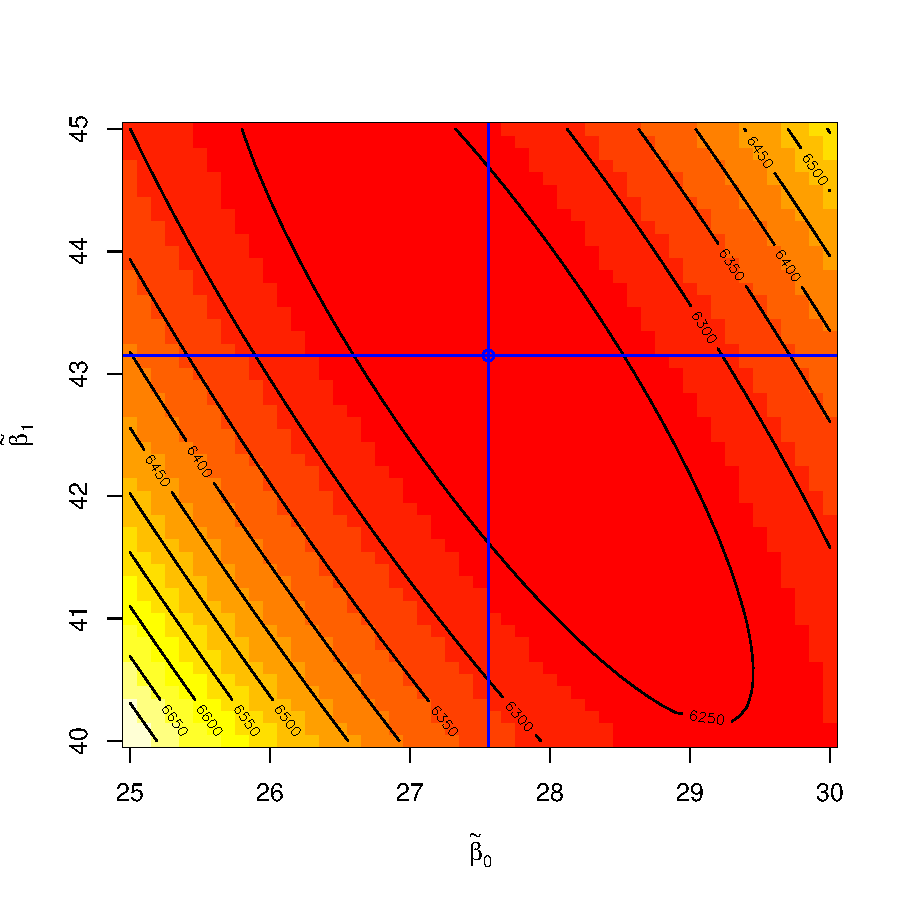
\includegraphics{OLSobjectiveFunction3.pdf}}
%\end{figure}
%
%}


\frame{
\frametitle{Descriptive Interpretation}

\begin{figure}[ht] \centering
        \scalebox{.4}{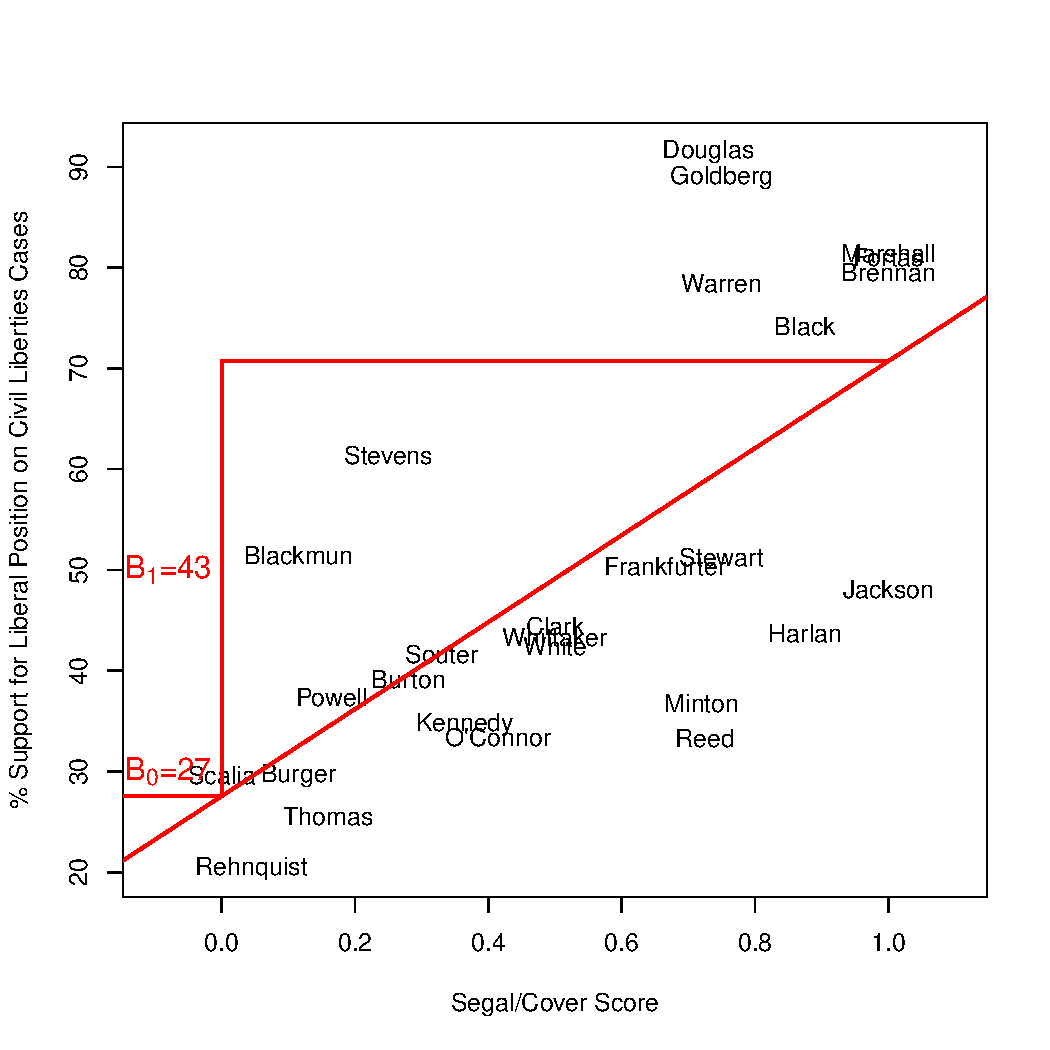
\includegraphics{lmPlot.pdf}}
\end{figure}
%$$
%\hat{\beta}_0 = 27.56 \text{ and } \hat{\beta}_1 = 43.15
%$$ 
}

%%%%%%%%%%%%%%
%\subsection{Goodness of Fit}

\frame{
\frametitle{Variance and Regression}

\begin{itemize}
\item Again, we want to assess the ``leastness'' of  least squares (i.e., the spread of the data around the line).
\item The standard error of the regression, $\sqrt{\frac{\sum_{i=1}^N e_i^2}{N-2}}$, is analogous to the standard deviation.
\item There are other approaches to this question: correlation and coefficient of determination.
\end{itemize}

}


\frame{
\frametitle{Covariance}

The population variances for $X$ and $Y$ can be written as:
\pause
\begin{align*}
S^2_{x} &= \frac{\sum_{i=1}^N (x_i-\bar{x})^2}{N-1} \\ \pause
&= \frac{\sum_{i=1}^N (x_i-\bar{x})(x_i-\bar{x})}{N-1}
\end{align*}
\pause
$$
S^2_{y} = \frac{\sum_{i=1}^N (y_i-\bar{y})(y_i-\bar{y})}{N-1}
$$


\visible<4->{What if we defined a similar quantity involving both $X$ and $Y$?}

\visible<5->{$$
S_{xy} = \frac{\sum_{i=1}^N (x_i-\bar{x})(y_i-\bar{y})}{N-1}
$$}

\visible<6->{This quantity is the \alert{covariance}.}

}

%\frame{
%\frametitle{Properties of Sample Covariance}
%
%	\begin{columns}
%		\begin{column}{.5\textwidth}
%$$
%s_{xy} = \frac{\sum_{i=1}^n (x_i-\bar{x})(y_i-\bar{y})}{n-1}
%$$
%
%\vspace{.15in}
%\pause
%Points in the upper right and lower left quadrants (relative to the means) add to the covariance.
%
%\vspace{.15in}
%\pause
%Points in the upper left and lower right quadrants subtract from the covariance.
%
%		\end{column}
%		\begin{column}{.5\textwidth}
%
%\begin{center}
%\includegraphics<1>[width=2in]{covbase.pdf}
%\includegraphics<2>[width=2in]{covpos.pdf}
%\includegraphics<3>[width=2in]{covneg.pdf}
%\includegraphics<4>[width=2in]{covend.pdf}
%\end{center}
%
%
%		\end{column}
%	\end{columns}
%
%}
%


\frame{
\frametitle{Correlation}

The covariance does not have units that are easy to interpret, so we can scale it by the standard deviations of $X$ and $Y$ to obtain the \alert{correlation}:

$$
R =\frac{S_{xy}}{S_{x}S_{y}}= \frac{\sum_{i=1}^N (x_i-\bar{x})(y_i-\bar{y})}{\sqrt{ \sum_{i=1}^N (x_i-\bar{x})^2  \sum_{i=1}^N (y_i-\bar{y})^2 }}
$$ 
\vspace{.2cm}

\pause
The correlation is always in the interval:
$$
-1 \le R \le 1
$$

}

\frame{
\frametitle{Analysis of Variance for the Regression}

How well do the Segal-Cover scores predict support for civil liberties in relation to the average support for civil liberties?
	\begin{columns}
		\begin{column}{.5\textwidth}
\begin{itemize}
\pause
\item  \textcolor{green}{$e_i = y_i -\widehat{y}_i$}
\pause
\item \textcolor{blue}{$y_i - \bar{y}$}
\pause
\item \textcolor{red}{$\widehat{y}_i - \bar{y}$}
\pause
\item \textcolor{blue}{$(y_i - \bar{y})$} $=$ \textcolor{green}{$e_i$} + \textcolor{red}{$(\widehat{y}_i - \bar{y})$}
\end{itemize}
		\end{column}
		\begin{column}{.5\textwidth}

\begin{center}
	\includegraphics<1>[width=2in]{emlmline.pdf}
	\includegraphics<2>[width=2in]{emresid.pdf}
	\includegraphics<3>[width=2in]{emmeandev.pdf}
	\includegraphics<4>[width=2in]{empred.pdf}
	\includegraphics<5>[width=2in]{emall.pdf}
\end{center}

		\end{column}
	\end{columns}

}

\frame{

\begin{eqnarray*}
\alert<6>{\sum_{i=1}^N(y_i - \bar{y})^2} &=& \sum_{i=1}^N \{e_i + (\widehat{y}_i - \bar{y})\}^2\\
\visible<2->{ &=& \sum_{i=1}^N \{e_i^2 + 2e_i (\widehat{y}_i - \bar{y})+ (\widehat{y}_i - \bar{y})^2\}}\\
\visible<3->{ &=& \sum_{i=1}^N e_i^2 + 2\sum_{i=1}^Ne_i (\widehat{y}_i - \bar{y})+ \sum_{i=1}^N(\widehat{y}_i - \bar{y})^2}\\
\visible<4->{ &=& \alert<7>{\sum_{i=1}^N e_i^2} + \alert<8>{\sum_{i=1}^N(\widehat{y}_i - \bar{y})^2}}\\
\visible<5->{\alert<6>{TSS} &=& \alert<7>{SSR} + \alert<8>{RegSS}}
\end{eqnarray*}

}

\frame{
\frametitle{Coefficient of Determination}

We can divide each side by the TSS:
$$
 \frac{SSR}{TSS} + \frac{RegSS}{TSS} = \frac{TSS}{TSS}
$$
\pause
$$
\frac{SSR}{TSS} + \frac{RegSS}{TSS} = 1
$$
\pause
$$
\frac{RegSS}{TSS} = 1 - \frac{SSR}{TSS} = \alert{R^2}
$$
\pause
$R^2$ is a measure of how much of the variation in $Y$ is accounted for by $X$.
}


\frame{
\frametitle{Usefull Identities}


$$
R^2 = (R)^2
$$

\pause
\begin{eqnarray*}
B_1 &=& \frac{\sum_{i=1}^N (x_i - \bar{x})(y_i -
  \bar{y})}{\sum_{i=1}^N(x_i - \bar{x})^2} \\ 
  & \visible<3->{=}&   \visible<3->{\frac{\sum_{i=1}^N (x_i-\bar{x})(y_i-\bar{y})}{\sqrt{ \sum_{i=1}^N (x_i-\bar{x})^2  \sum_{i=1}^Nn (y_i-\bar{y})^2 }} \cdot \frac{\sqrt{\frac{\sum_{i=1}^N (y_i-\bar{y})^2}{N-1}}}{\sqrt{\frac{\sum_{i=1}^N (x_i-\bar{x})^2}{N-1}}} }\\
  & \visible<4>{=}& \visible<4>{R\frac{S_y}{S_x}}
\end{eqnarray*}

}

\frame{

	\begin{columns}
		\begin{column}{.5\textwidth}

\begin{itemize}

\item $R^2 = 0.45$
\item $R = \sqrt{R^2} = 0.67$
\item $S_x = 0.33$
\item $S_y = 20.9$
\item $B_1 = R\frac{S_y}{S_x} = 43.15$
\end{itemize}

		\end{column}
		\begin{column}{.5\textwidth}

\begin{figure}[ht] \centering
        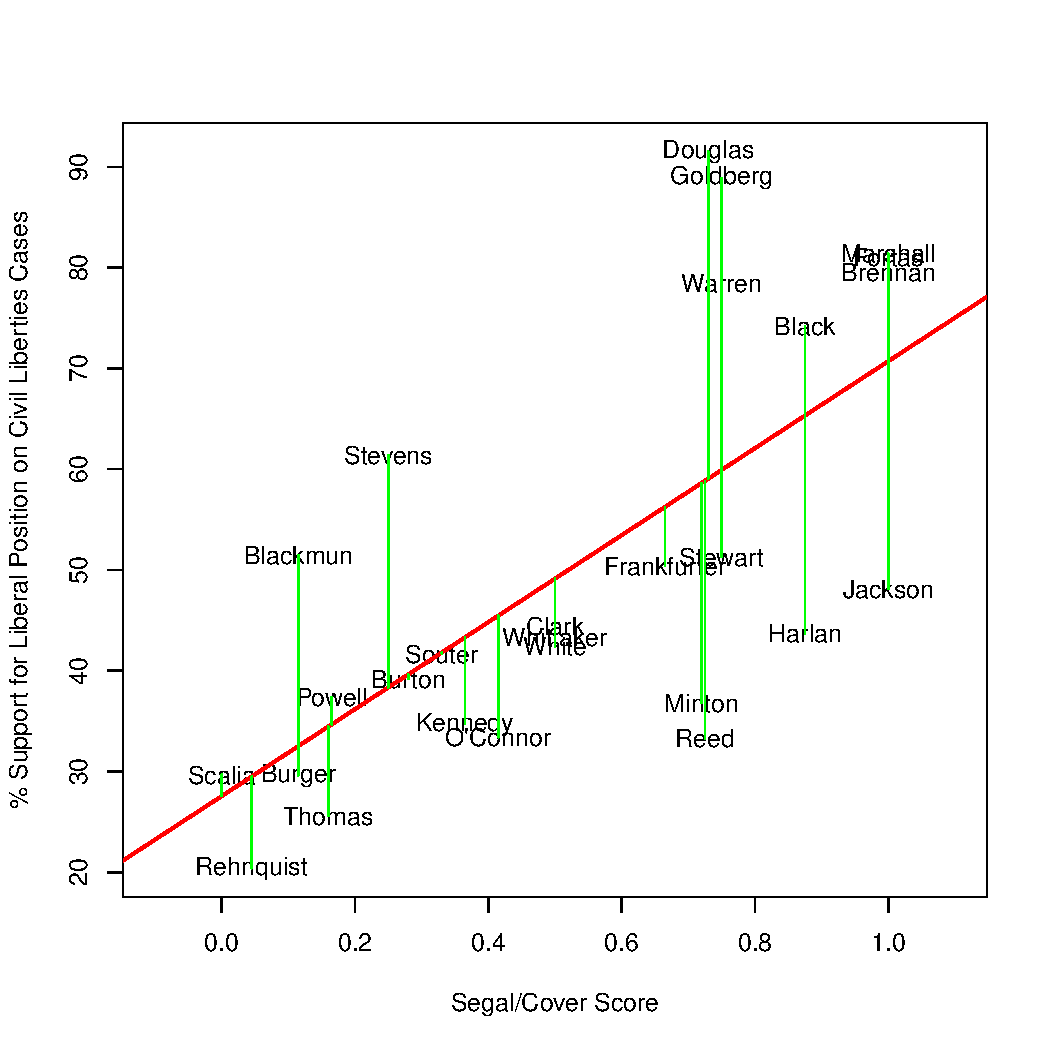
\includegraphics[width=2in]{residuals.pdf}
\end{figure}
		\end{column}
	\end{columns}
}

\frame{
\frametitle{Anscombe's Quartet}

\begin{figure}[ht] \centering
        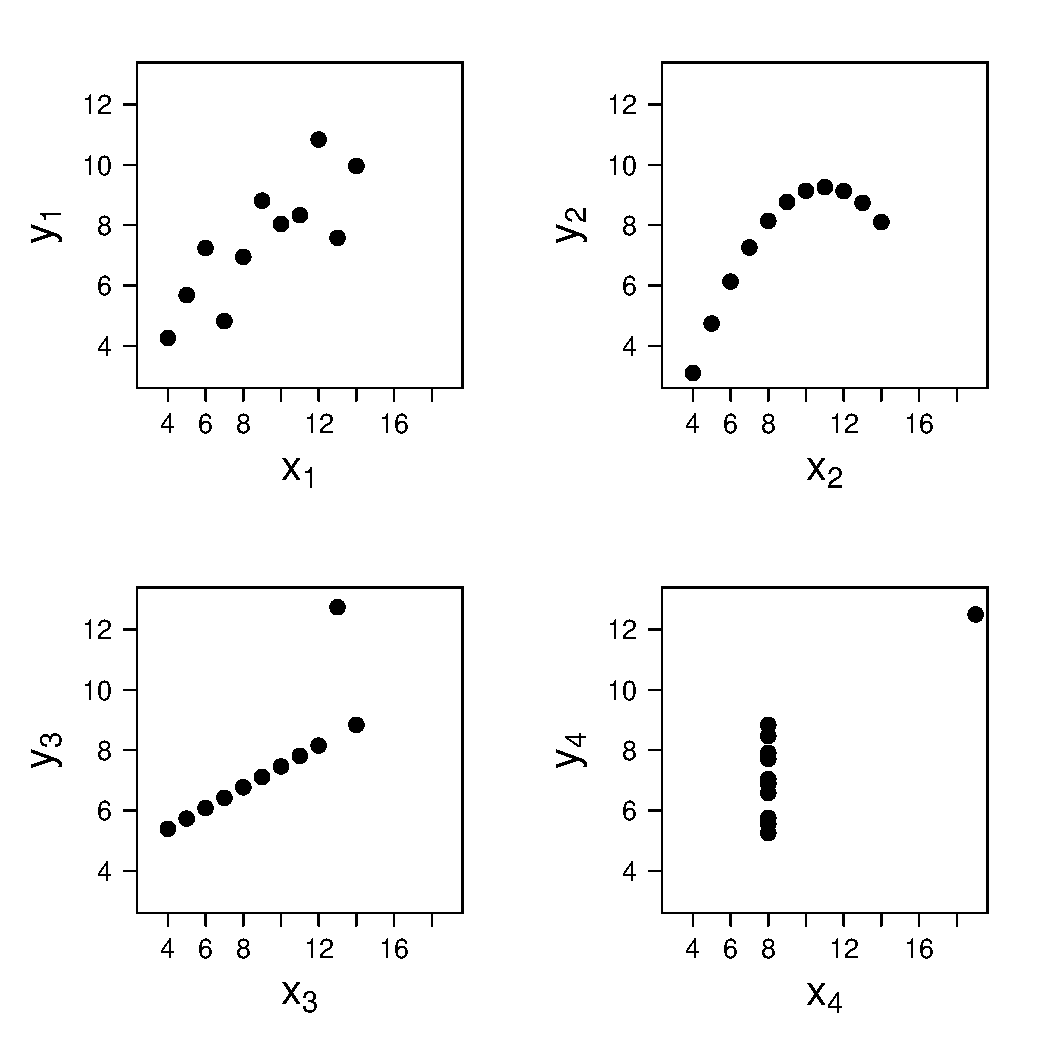
\includegraphics[width=3in]{Anscombe.pdf}
\end{figure}

}

\frame{

	\begin{columns}
		\begin{column}{.5\textwidth}

\begin{figure}[ht] \centering
        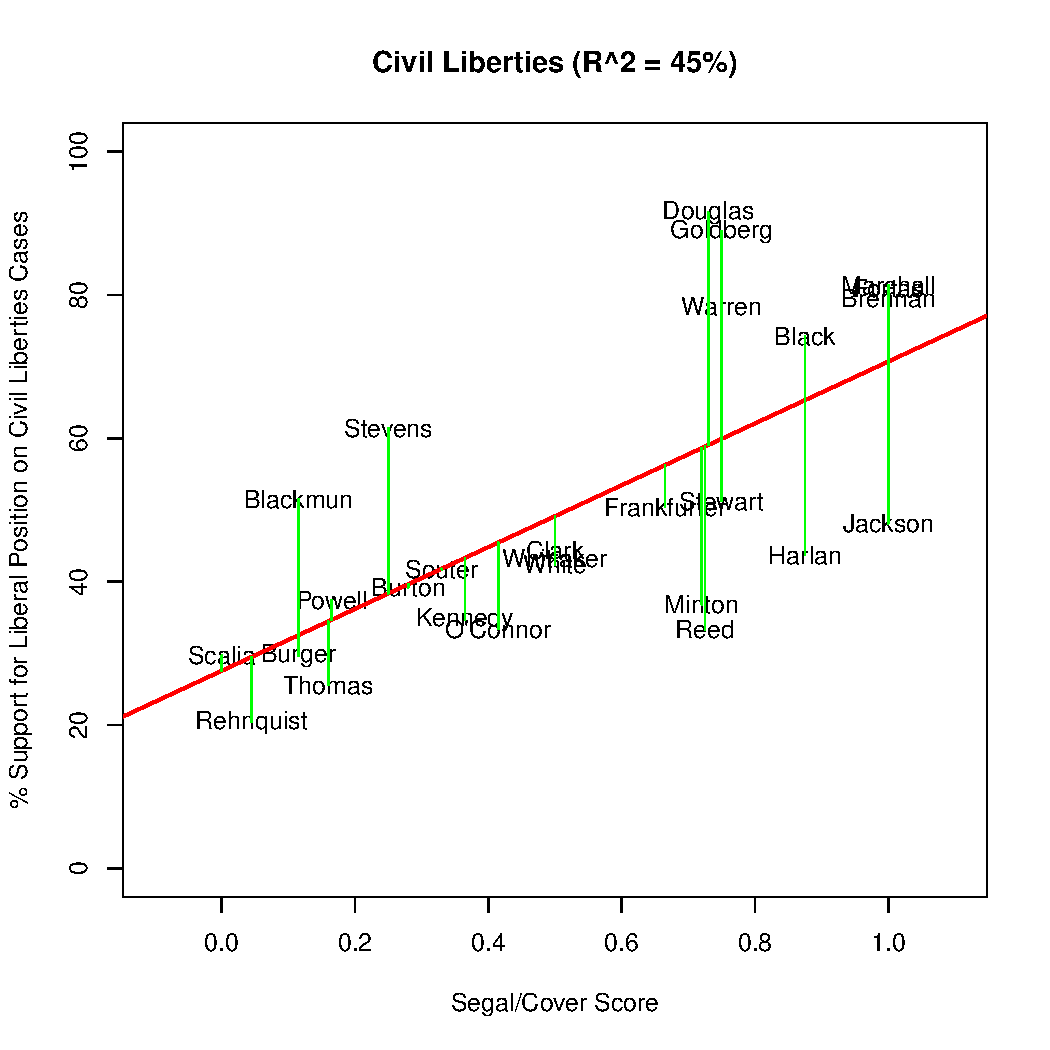
\includegraphics[width=2in]{residuals1.pdf}
\end{figure}
		\end{column}
		\begin{column}{.5\textwidth}

\begin{figure}[ht] \centering
        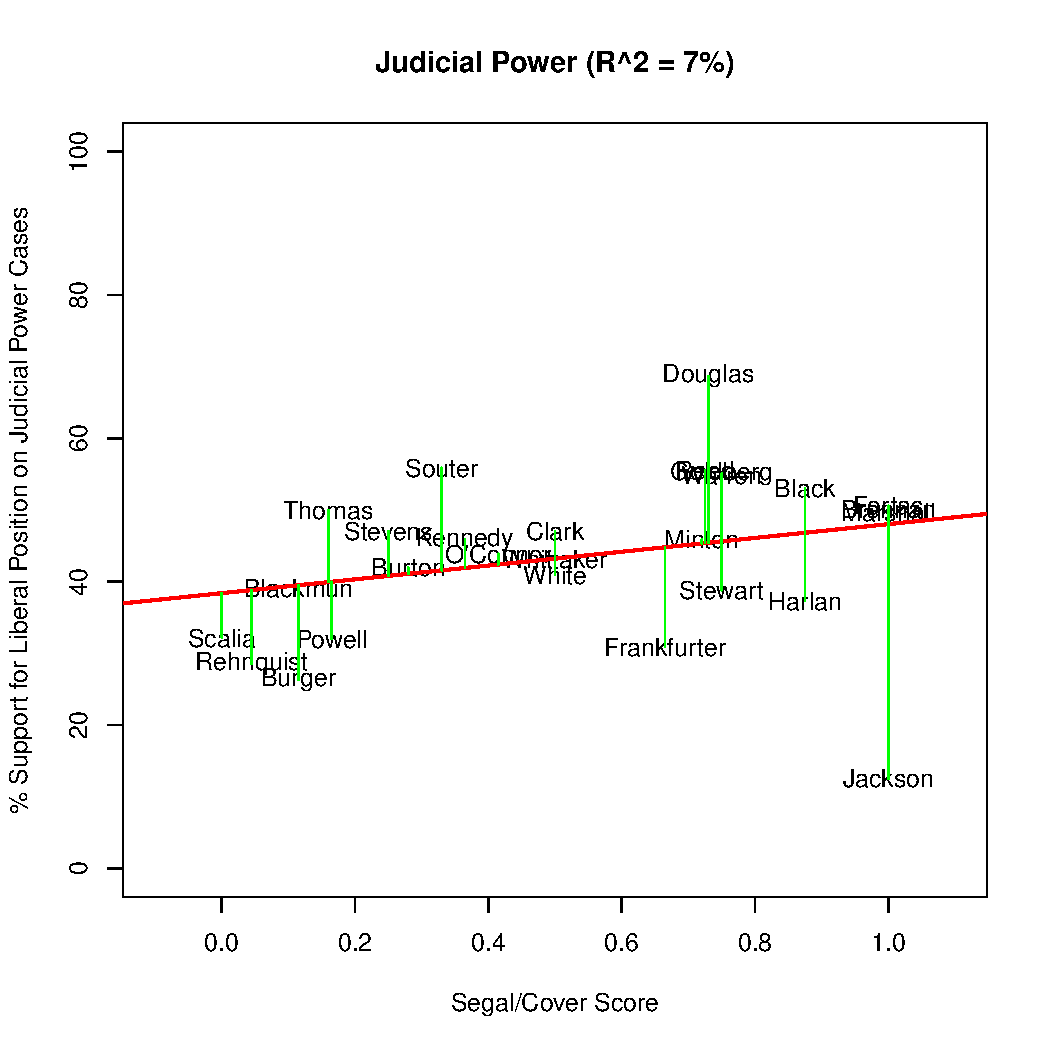
\includegraphics[width=2in]{residuals3.pdf}
\end{figure}
		\end{column}
	\end{columns}
}



%\frame{
%	\frametitle{Question:}

%Assume that X and Y are measured in the same units.  Under what conditions will the least squares slope from the regression of Y on X be the same as the least squares slope from the regression of X on Y?

%\begin{itemize}
%\item [A)] The slopes are the same when $s_x = s_y$.
%\item [B)]The slopes are the same when $r = \frac{s_y}{s_x}$.
%\item [C)]The slopes are the same when $s_x = 1$.
%\item [D)]The slopes are never the same.
%\end{itemize}
%}


%%%%%%%%%%%%%%%%%%%%


\section{Description with Multiple Regression}


\frame{
\frametitle{More Than One Conditioning Variable}

\begin{itemize}
\item Often we want averages conditional on more than one variable.
\item As with continuous conditioning variables, there are many ways to do this.
\item In this class we will look at two.
\end{itemize}


}

\frame{
\frametitle{Multiple Regression with 2 Conditioning Variables}

\begin{itemize}
\item Fitted Values from the LCMF $\hat{y}_i = B_0 + B_1 x_i + B_2 z_i$\\
 for $i=1,...,N$ \pause
\item Residuals from Fitted Values:  $e_i = y_i - \hat{y}_i$ for $i=1,...,N$
\end{itemize} \pause

\vspace{.5cm}

Again, we choose $B_0$, $B_1$, and $B_2$, to minimize the SSR, where
\begin{align*}
SSR &= \sum_{i=1}^N e_i^2
\end{align*}
but the definition of $e_i$ changes with the inclusion of more variables. 
}
\frame{
\frametitle{One Binary and One Continuous Conditioning Variable}

\begin{figure}[ht] \centering
        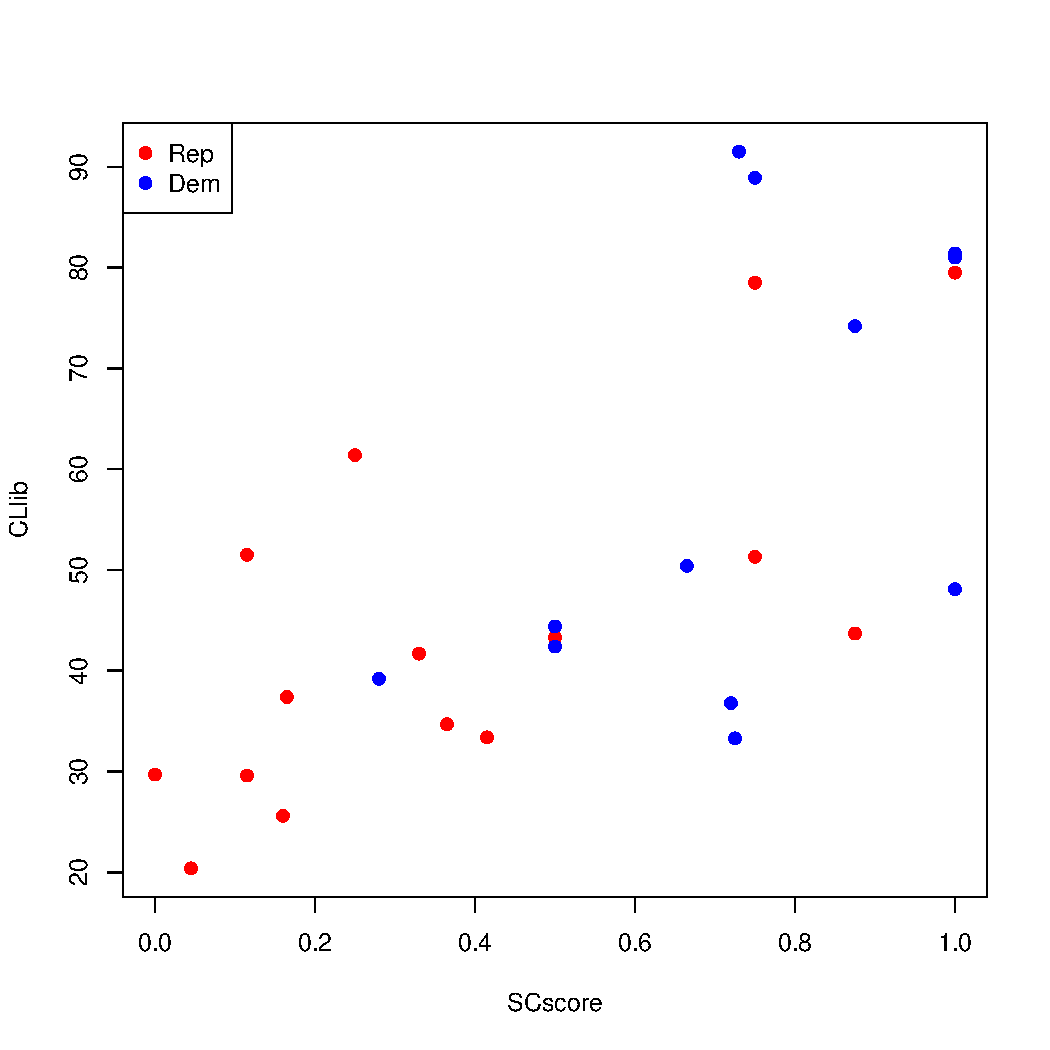
\includegraphics[width=3in]{psc.pdf}
\end{figure}

}

\frame{
\frametitle{One Binary and One Continuous Conditioning Variable}

\begin{figure}[ht] \centering
        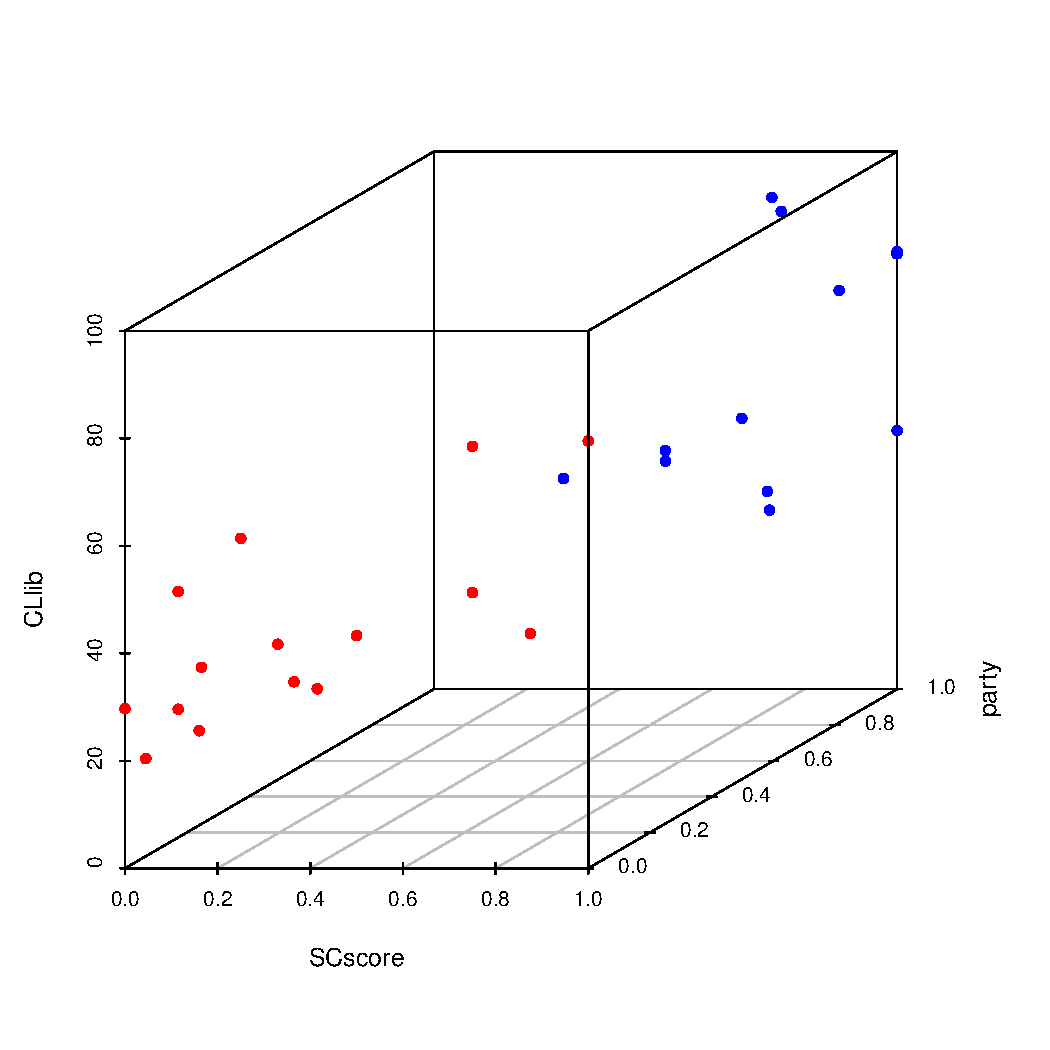
\includegraphics[width=3in]{em3D1.pdf}
\end{figure}
}

\frame{
\frametitle{One Binary and One Continuous Conditioning Variable}

\begin{figure}[ht] \centering
        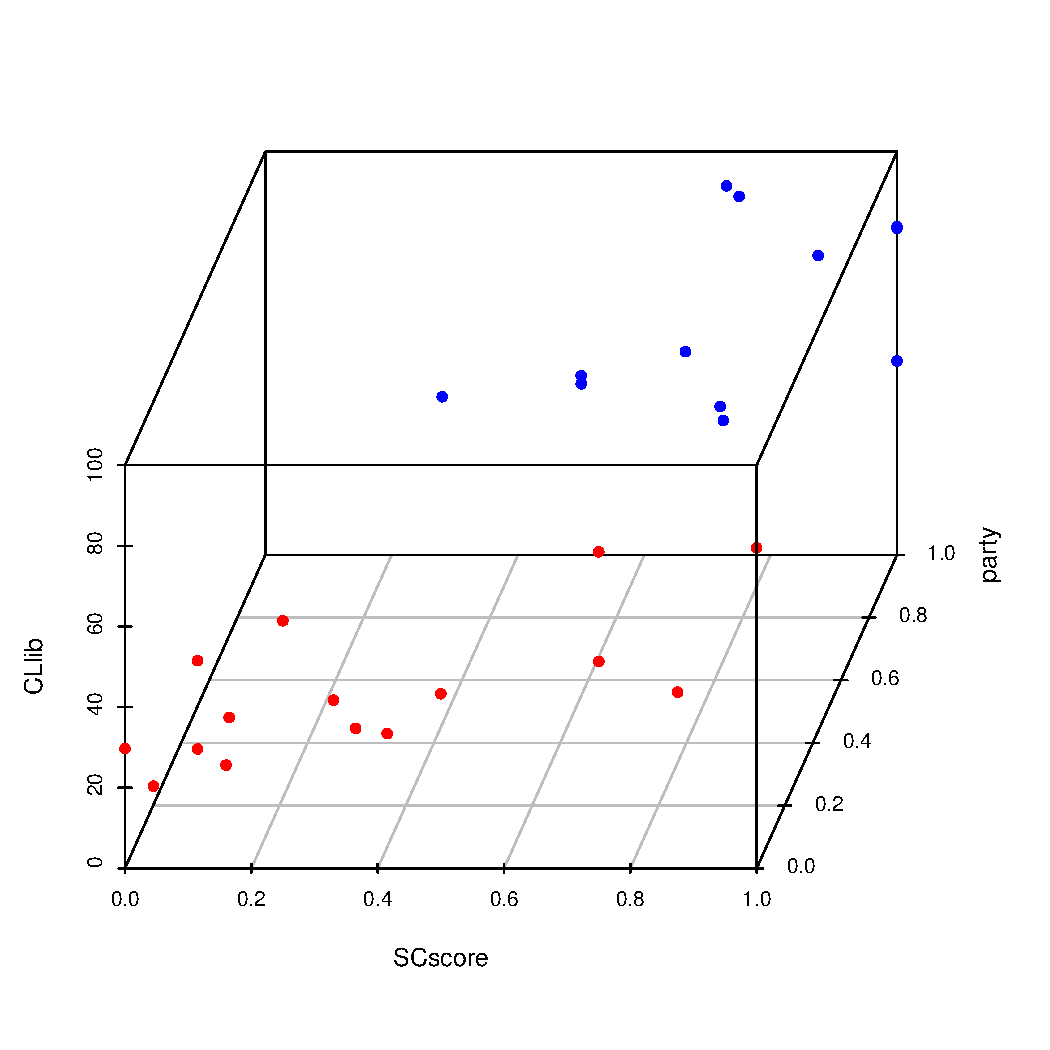
\includegraphics[width=3in]{em3D2.pdf}
\end{figure}
}

\frame{
\frametitle{Regression Plane}
\begin{figure}[ht] \centering
        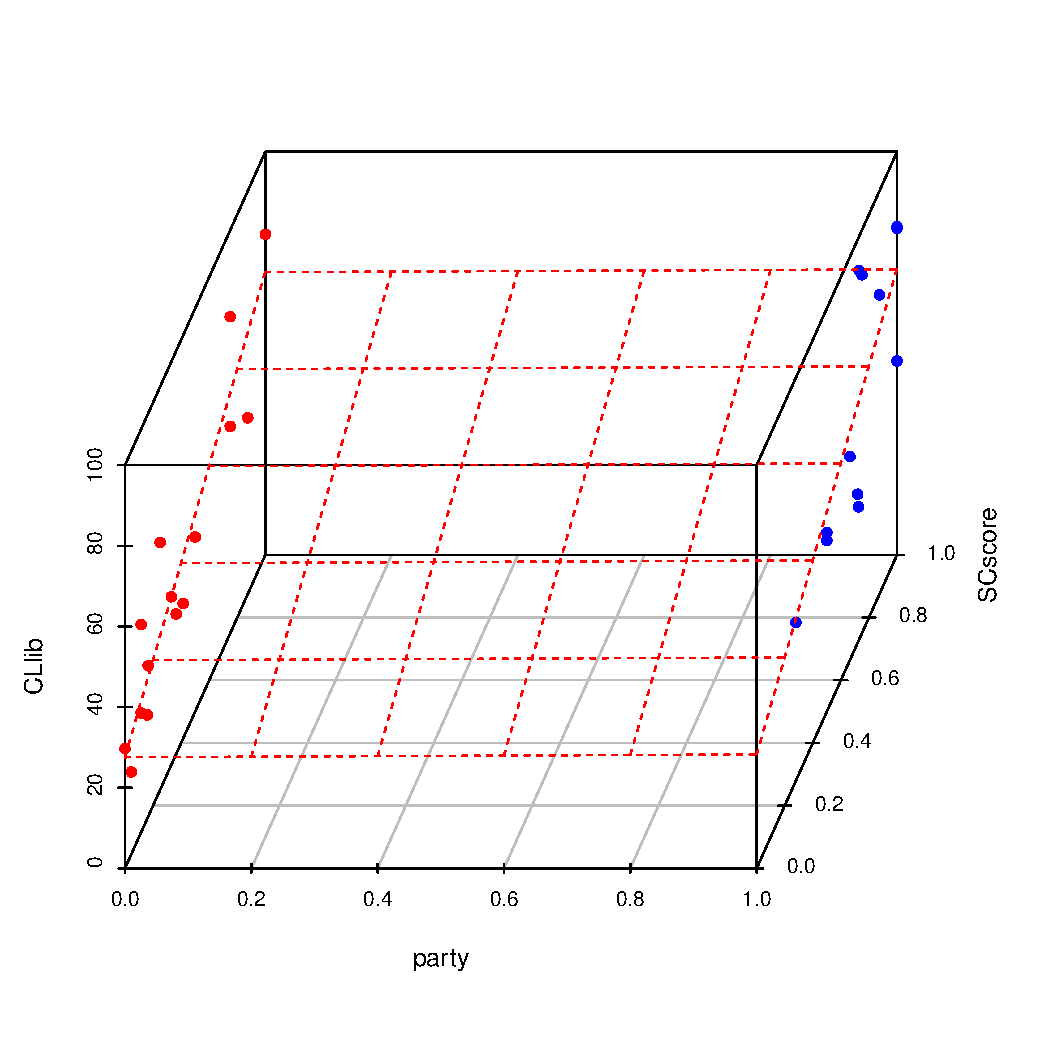
\includegraphics[width=3in]{em3D3.pdf}
\end{figure}
}

\frame{
\frametitle{Multiple Regression Activity}
Draw the two regression lines (i.e., edges of the regression plane) implied by 
$$
\hat{y} = B_0 + B_1 x + B_2 z
$$
\begin{figure}[ht] \centering
        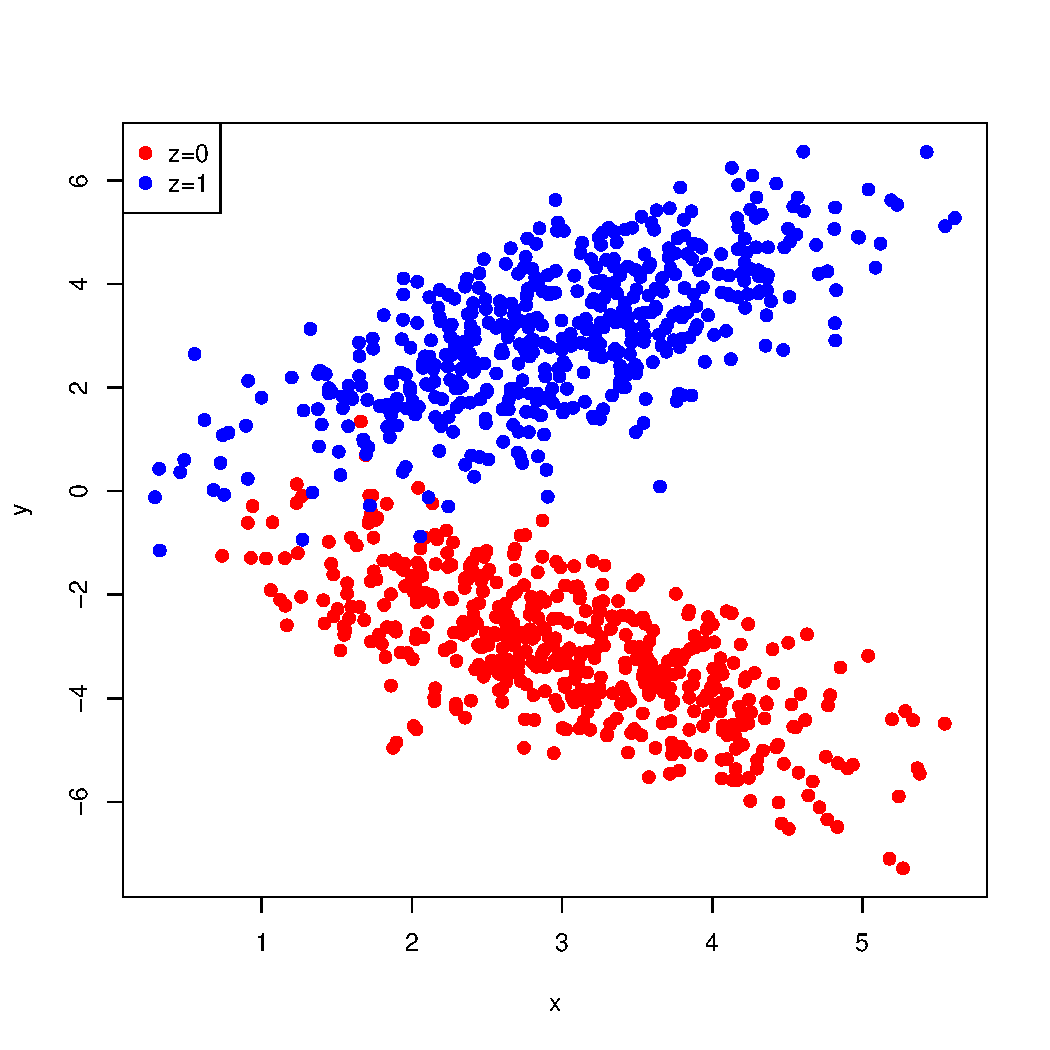
\includegraphics[width=2.5in]{multAct.pdf}
\end{figure}

}

\frame{
\frametitle{Multiple Regression Activity}
Draw the two regression lines (i.e., edges of the regression plane) implied by 
$$
\hat{y} = B_0 + B_1 x + B_2 z
$$
\begin{figure}[ht] \centering
        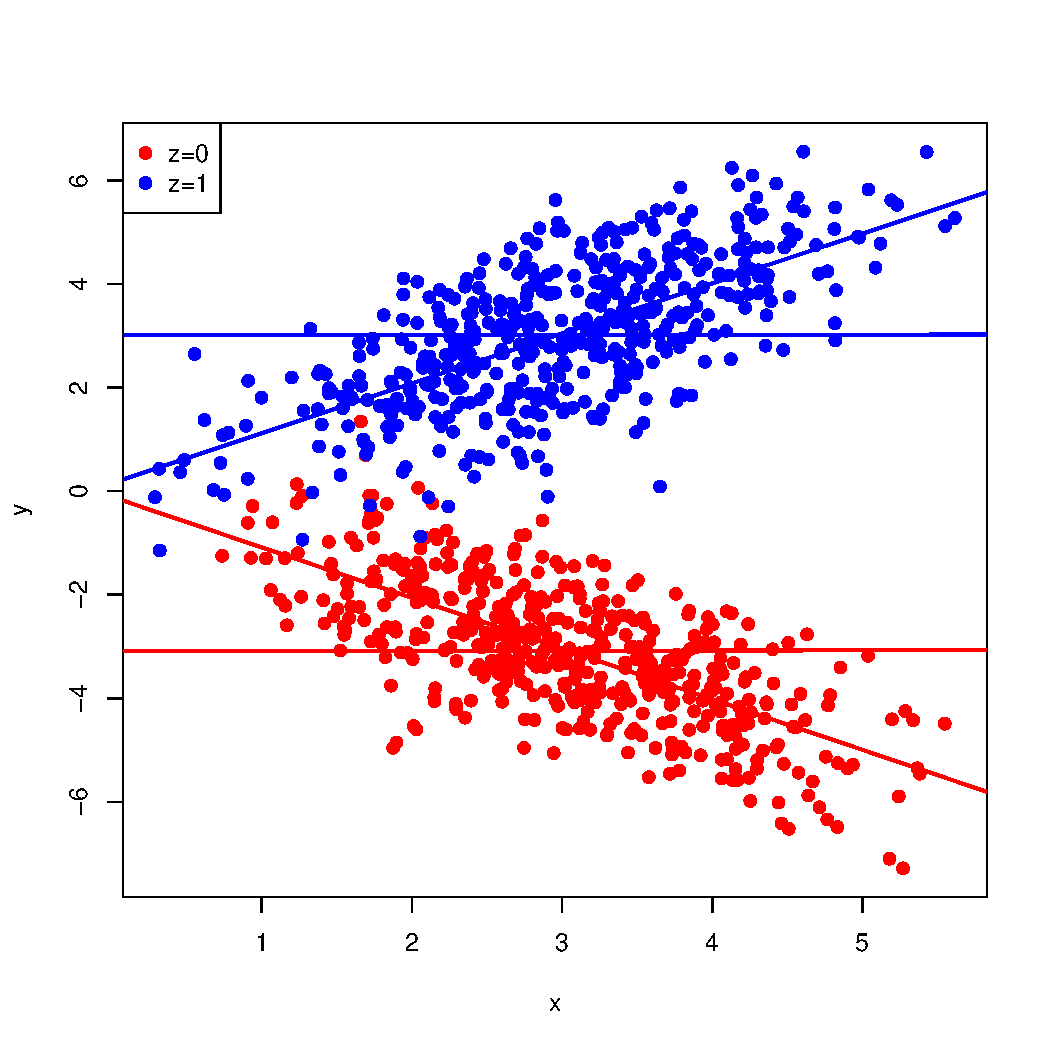
\includegraphics[width=2.5in]{multActSol.pdf}
\end{figure}

}


\frame{
\frametitle{Regression Plane for Two Continuous Conditioning Variables}

\begin{figure}[ht] \centering
        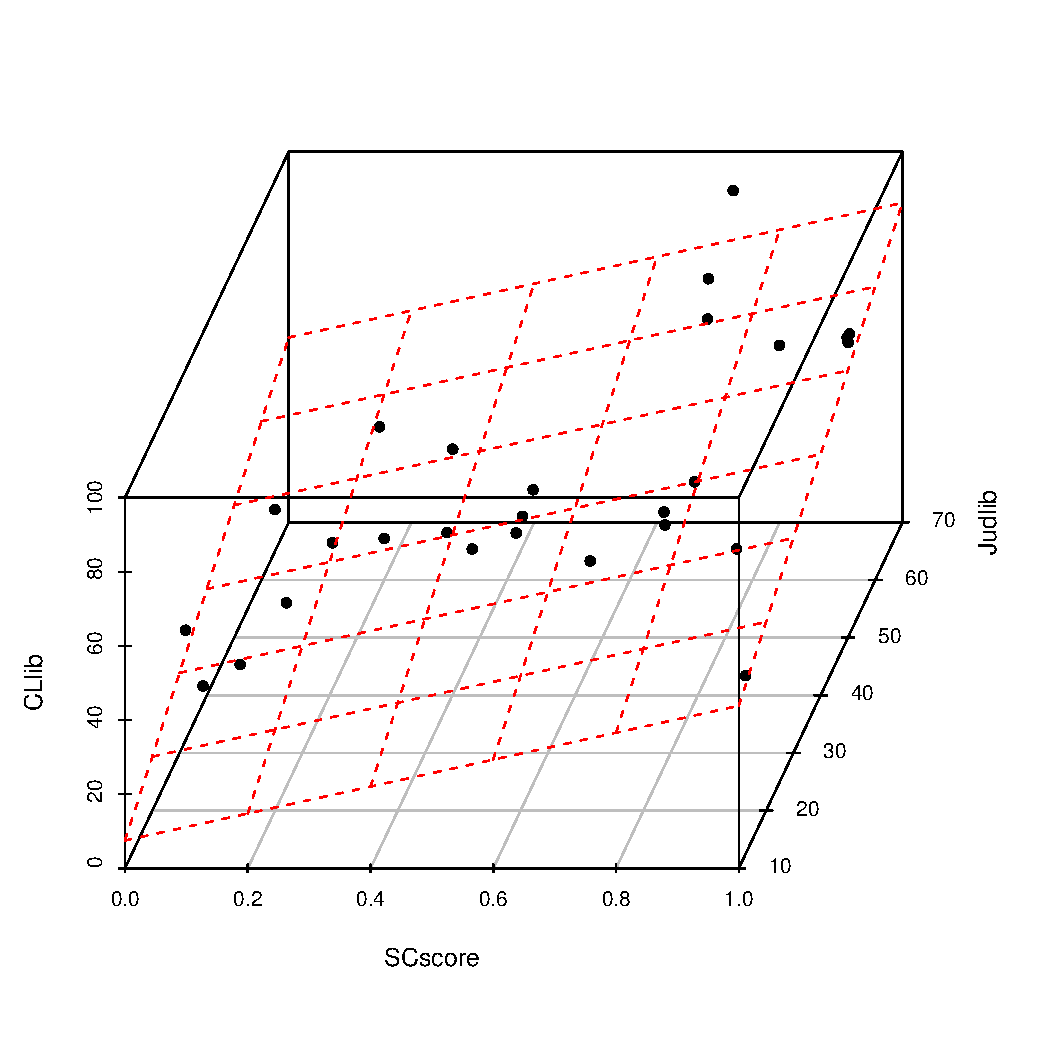
\includegraphics[width=3in]{em3D4.pdf}
\end{figure}
}


\frame{
\frametitle{Descriptive Interpretation of Additive Regression}

$$\widehat{CLlib}_i = B_0 + B_1 \cdot SCscore_i + B_2 \cdot Dem_i$$

\begin{figure}[ht] \centering
        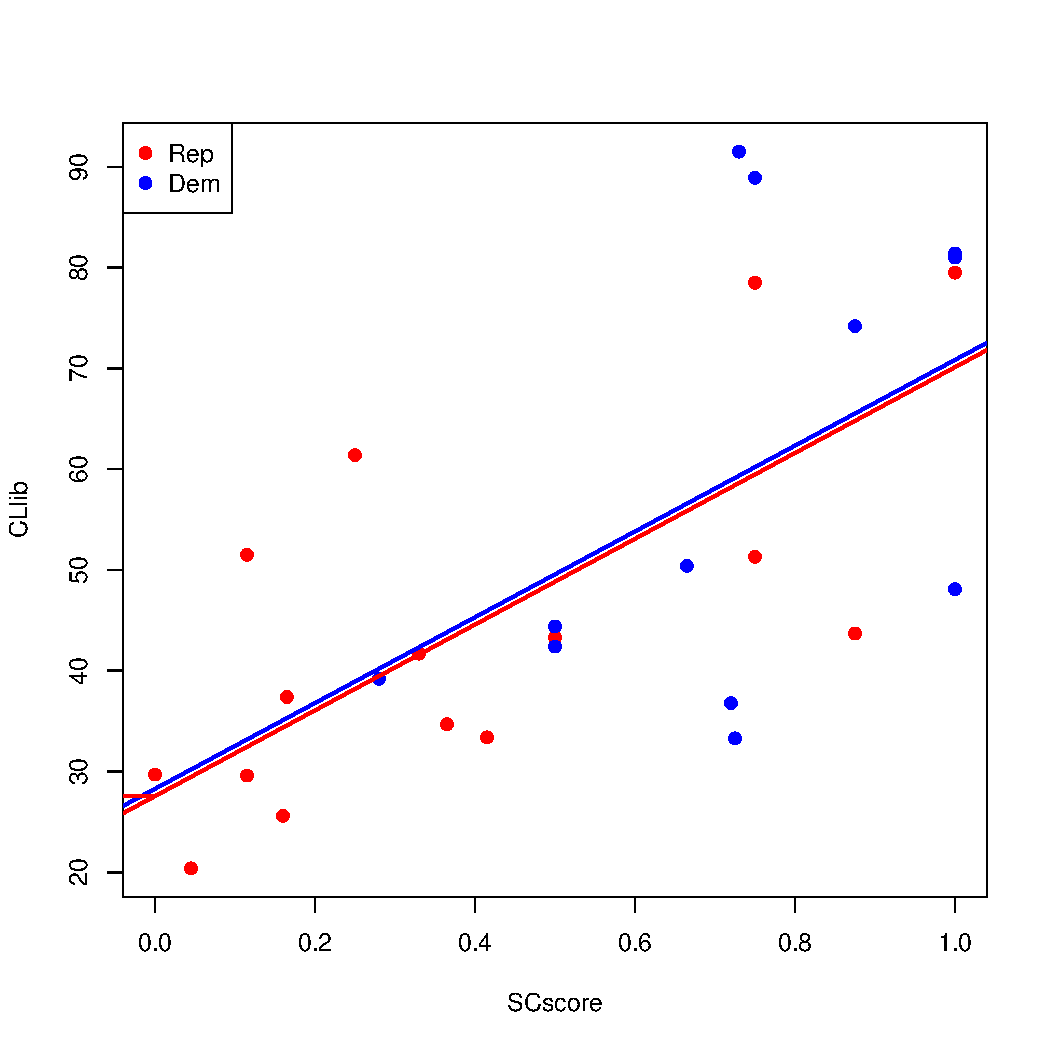
\includegraphics[width=2.7in]{pscMarg.pdf}
\end{figure}

}

\frame{
\frametitle{Descriptive Interpretation of Additive Regression}

$$\widehat{Fedlib}_i = B_0 + B_1 \cdot SCscore_i + B_2 \cdot Dem_i$$

\begin{figure}[ht] \centering
      \includegraphics<1>[width=2.7in]{pscMarg2.pdf}
	\includegraphics<2>[width=2.7in]{pscMarg20.pdf}
	\includegraphics<3>[width=2.7in]{pscMarg21.pdf}
	\includegraphics<4>[width=2.7in]{pscMarg22.pdf}
	\end{figure}

}


\frame{
\frametitle{Multiple Regression with an Interaction}

\begin{itemize}
\item Fitted Values: $\hat{y}_i = B_0 + B_1 x_i + B_2 z_i + B_3 x_i \cdot z_i$ \\
for $i=1,...,N$ \pause
\item Residuals:  $e_i = y_i - \hat{y}_i$ for $i=1,...,N$
\end{itemize} \pause

\vspace{.5cm}

Again, we choose $B_0$, $B_1$, $B_2$, and $B_3$, to minimize the SSR, where
\begin{align*}
SSR &= \sum_{i=1}^N e_i^2
\end{align*}
but the definition of $e_i$ has again changed. 
}




\frame{
\frametitle{Descriptive Interpretation of Interaction Model}

$$\widehat{Fedlib}_i = B_0 + B_1 \cdot SCscore_i + B_2 \cdot Dem_i + B_3 \cdot SCscore_i \cdot Dem_i$$

\begin{figure}[ht] \centering
      \includegraphics<1>[width=2.7in]{pscInt.pdf}
	\includegraphics<2>[width=2.7in]{pscInt0.pdf}
	\includegraphics<3>[width=2.7in]{pscInt1.pdf}
	\includegraphics<4>[width=2.7in]{pscInt2.pdf}
	\includegraphics<5>[width=2.7in]{pscInt3.pdf}

\end{figure}
%
}

\frame{
\frametitle{Variance and Multiple Regression}

\begin{itemize}
\item As before, we want to assess the ``leastness'' of  least squares (i.e., the spread of the data around the plane or twisted plane).
\item The standard error of the regression, $\sqrt{\frac{\sum_{i=1}^N e_i^2}{N-k}}$, now accounts for the number of $B$'s in the model (where $k$ is the number of $B$'s).
\item $R^2$ uses the same formula $1-\frac{SSR}{TSS}$, however the inclusion of additional variables will automatically reduce the SSR. 
\end{itemize}

}



\frame{
\frametitle{Summary Activity}

\begin{figure}[ht] \centering
      \includegraphics<1>[width=2.7in]{finalAct.pdf}
	\includegraphics<2>[width=2.7in]{finalAct1.pdf}
	\includegraphics<3>[width=2.7in]{finalAct2.pdf}
	\includegraphics<4>[width=2.7in]{finalAct3.pdf}
	\includegraphics<5>[width=2.7in]{finalAct4.pdf}
\end{figure}

}

%\frame{
%\frametitle{Summary}
%
%\begin{itemize}
%\item There are many possible descriptive questions with many variables and variables that take many values. 
%\item In this course we focus on means (possibly conditional), although variance and standard deviation are also concerns. 
%\item Conditioning requires modeling choices. In this course we use linear models (with and without interactions). 
%\end{itemize}
%
%}
%
%\frame{
%\frametitle{Next Week}
%
%Randomly Sampled Observations and Basic Probability
%
%\begin{itemize}
%\item Elementary Probability Theory
%\item Random Variables and Functions of Random Variables (Expectation, Variance, ...)
%\item Joint and Conditional Distributions
%\end{itemize}
%
%\vspace{.5cm}
%
%Things to do:
%\begin{itemize}
%\item first problem set
%\item the reading and the reading quiz
%\item annotations (if you have a question or want to respond to a question)
%\end{itemize}
%
%
%
%}



\end{document}












